\documentclass{xtufte-handout}
\usepackage{fontspec}

\setmainfont{Noto Sans}
\newfontfamily{\tam}[Script=Tamil]{Noto Sans Tamil}
\title{Sound\thanks{Draft version as of \today}}
\author{Disha Kuzhively\thanks{disha.jk@icts.res.in}}
\date{\today}
% \geometry{showframe}   

\usepackage{graphicx} % allow embedded images
  \setkeys{Gin}{width=\linewidth,totalheight=\textheight,keepaspectratio}
\usepackage{fancyvrb} % extended verbatim environments
  \fvset{fontsize=\normalsize}% default font size for fancy-verbatim environments  
\usepackage{booktabs}
\usepackage{tikz}
\usepackage[none]{hyphenat}
\usepackage{xkcdcolors}
% Standardize command font styles and environments
\newcommand{\doccmd}[1]{\texttt{\textbackslash#1}}% command name -- adds backslash automatically
\newcommand{\docopt}[1]{\ensuremath{\langle}\textrm{\textit{#1}}\ensuremath{\rangle}}% optional command argument
\newcommand{\docarg}[1]{\textrm{\textit{#1}}}% (required) command argument
\newcommand{\docenv}[1]{\textsf{#1}}% environment name
\newcommand{\docpkg}[1]{\texttt{#1}}% package name
\newcommand{\doccls}[1]{\texttt{#1}}% document class name
\newcommand{\docclsopt}[1]{\texttt{#1}}% document class option name
\newenvironment{docspec}{\begin{quote}\noindent}{\end{quote}}% comm
\newcommand{\hertz}{Hz}

\tikzset{
    pencil/.pic={
        \pgfmathsetmacro{\l}{3}
        \pgfmathsetmacro{\w}{\l/10}
        % Pencil body
        \fill[orange!80!yellow] (0,0) rectangle (\l,\w);
        % Wooden sharpened part
        \fill[brown!30] (\l,0) -- ({7*\l/6},\w/2) -- (\l,\w) -- cycle;
        
        \fill[black] ({7*\l/6},{\w/2}) -- ($({7*\l/6},{\w/2})!0.3!(\l,\w)$) --($({7*\l/6},{\w/2})!0.3!(\l,0)$) --cycle;
        % Edge lines

        \draw (0,0) rectangle (\l,\w);

        \draw (\l,0) -- ({7*\l/6},\w/2) -- (\l,\w);
        \fill[pink!60,draw=black] (-\w,0) rectangle (0,\w);
        \fill[gray!50, draw=black] (-\w/3,0) rectangle (0,\w);
    },
    speaker/.pic={
        \draw (-1,-1) --++ (0.5,0) --++ (1.5,-1)--++(0,3)--++(-1.5,-1)--++(-0.5,0);
        \node[text width=2cm] at (0,-.5) {Source of sound}; 
    }
}
\begin{document}
\maketitle

\begin{abstract}
\noindent
This article was prepared by the author to serve as a draft for the TNSCERT class 8 chapter on the concept of Sound during the the Tamil Nadu Curriculum Framing (TNCF) workshops that were held in Asha Nivas, Chennai from 13-11-2025 to 15-11-2025, and 09-03-2026 to 10-03-2026.
\end{abstract}

Every day we hear many natural and human-made sounds around us. At night, we may hear the soft noise of crickets. At dawn, the chirping of birds welcomes a new day. As the town wakes up, we hear buses, cars, two-wheelers, and the honking of horns. In school, the ringing of the bell tells us when a class begins or ends. We also hear raindrops falling on the ground, a dog barking, or a phone ringing.

Where do these sounds come from? In this chapter, we will explore how sound is produced and how it propagates from one place to another. We will also learn that sound can be understood as a wave.

\newthought{Exercise:} Close your eyes for one minute and listen carefully. Write down all the sounds you hear.
\section{Activity: Vibrating Scale}
\subsection{Materials required}
\begin{enumerate}
    \item Scale
\item Desk or table
\end{enumerate}
\subsection{Procedure}
Place the scale on the desk so that about one-third of it is over the edge. Hold the part on the desk firmly with one hand. Push the free end of the scale downward. Release it quickly.
\begin{marginfigure}[-20\baselineskip]
  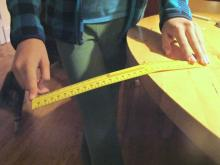
\includegraphics{scale-down}
  \caption[Sound with a scale]{Step 1. Push the free end of the scale downwards.}
\end{marginfigure}
\marginnote{\footnotesize Image credit: Ingrid Sulston, licensed under CC BY-NC-SA 4.0}
\begin{marginfigure}
  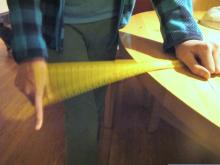
\includegraphics{scale-vibrate}
  \caption[Sound with a scale]{Step 2. Let the pushed end go.}
\end{marginfigure}
\marginnote{\footnotesize Image credit: Ingrid Sulston, licensed under CC BY-NC-SA 4.0}
\newthought{Observe} the movement of the scale. Do you hear a sound? Do you see the scale move up and down rapidly? What type of motion is this?
\section{Activity: Rubber Band Instrument}
\subsection{Materials required}
\begin{enumerate}
\item Rubber bands
\item Geometry box or pencil box
\item Two pens or pencils
\end{enumerate}
\subsection{Procedure}
Close the geometry box or pencil box. Stretch a rubber band around the box so that it lies across the top surface. Place a pen or pencil under the rubber band near one end of the box. Place another pen or pencil under the rubber band near the other end of the box. This will lift the rubber band slightly above the surface of the box. See Figure 3. Pluck the rubber band with your finger.
\begin{marginfigure}
  \centering
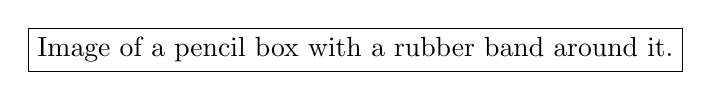
\begin{tikzpicture}
    \node[draw] at (0,0) {Image of a pencil box with a rubber band around it.};
  \end{tikzpicture}
  \caption{\label{rubberbox}Pencil box with rubber band around it.}
\end{marginfigure}
\newthought{Observe} the movement of the rubber band. Do you hear a sound? What part of the setup is moving?

\section{Activity: Tuning Fork}
\begin{marginfigure}
  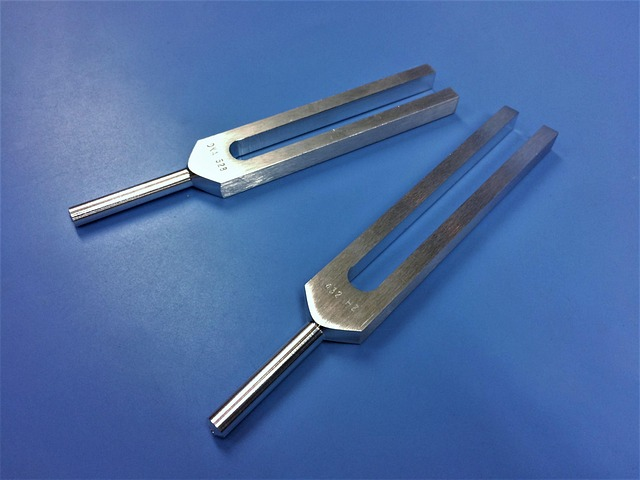
\includegraphics{tuning-fork}
  \caption[Tuning fork]{Tuning fork}
\end{marginfigure}
\subsection{Materials required}
\begin{enumerate}
\item Tuning fork
\item Rubber hammer
\item Bowl of water
\end{enumerate}
\subsection{Procedure}
Hold the tuning fork by its stem. Strike one prong of the tuning fork gently with a rubber hammer. Bring the vibrating tuning fork close to your ear.
\newthought{Observe:} Can you hear a sound? Touch the vibrating prongs gently with your finger. What do you feel when you touch the prongs? Touch the vibrating prongs lightly to the surface of the water. Observe the surface of the water. Do you see ripples on the surface of the water?
\begin{marginfigure}
  \centering
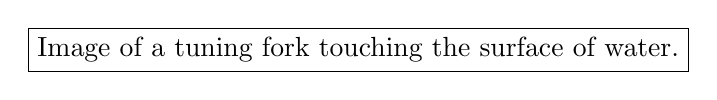
\begin{tikzpicture}
    \node[draw] at (0,0) {Image of a tuning fork touching the surface of water.};
  \end{tikzpicture}
  \caption{Ripples are formed on the surface of water when a vibrating tuning fork touches it.}
  \label{tuning-fork-water}
\end{marginfigure}

\marginnote{Did you know? Many quartz clocks and watches keep time using a small quartz crystal. This crystal is shaped like a tiny tuning fork.}

In these activities, we notice that sound is produced whenever there is \textbf{vibration}. The type of motion where there is a rapid back and forth or up and down motion is called vibration.

\section{Activity: Sound from a Iron Rod / School Bell}
\subsection{Materials required}
\begin{enumerate}
\item A hanging iron rod or a school bell
\item A hammer
\end{enumerate}
\subsection{Procedure}
Strike the hanging iron rod/bell gently with the hammer. Listen to the sound produced. Touch the rod/bell gently with your finger. Do you feel any vibrations? Do you hear the bell ringing? Hold the rod/bell firmly with both hands and not let it move. Do you feel any vibrations now? Do you hear a buzzing sound?
\begin{marginfigure}
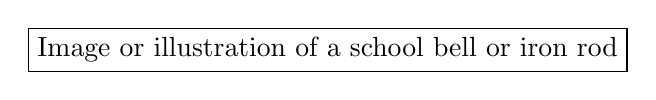
\begin{tikzpicture}
  \node[draw] at (0,0) {Image or illustration of a school bell or iron rod};
\end{tikzpicture}
  \caption{Image or illustration of a school bell or iron rod}
\end{marginfigure}
\subsection{Observe and record your observations}
\begin{fullwidth}
\begin{table}[h]
  \centering
  \begin{tabular}{lll}
    \toprule
    What you did & Did you feel any vibrations? & Did you hear a sound? \\
    \midrule
    Struck the bell and touched it gently & Yes / No &  Yes / No \\
    Held the bell firmly with both hands     & Yes / No &  Yes / No \\
    \bottomrule
  \end{tabular}
%   \caption{}
\end{table}
\end{fullwidth}

\newthought{Discuss} When did you hear the sound? When did the sound stop? What happened to the vibrations when you held the bell firmly?

In every activity, sound was produced only when something was moving. We notice that in the absense of any movement, no sound is produced.

\section{Activity: Pen Cap Instrument}
\subsection{Materials required}
A pen cap or marker cap
\subsection{Procedure}
Hold the pen cap by its sides. Place the open end of the cap just below your lower lip. Blow gently across the open end of the cap. Change the direction and strength of your breath until you hear a sound. Repeat the activity several times.
\newthought{Observe} Do you hear a sound? Is the pen cap moving? What is vibrating to produce the sound?
\begin{marginfigure}
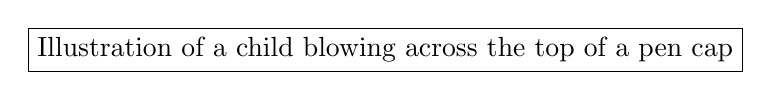
\begin{tikzpicture}
  \node[draw] at (0,0) {Illustration of a child blowing across the top of a pen cap};
\end{tikzpicture}
  \caption{Illustration of a child blowing across the top of a pen cap}
\end{marginfigure}
\subsection{Discussion}
Blowing across a pen cap produced a sound because the air inside the pen cap vibrated.

The vibrating part varied between activities.  In the scale, rubber band, tuning fork and school bell, a solid object vibrated.  In the pen cap, the air column inside vibrated. This shows that sound can also be produced by vibration of air.

\section{Sound from Musical Instruments}
Musical instruments also produce sound through a vibrating object inside them. In a guitar or veena, the strings vibrate. In a drum or a parai, the stretched membrane vibrates. In a Nadaswaram, flute, or a whistle, the air column inside the tube vibrates.
\begin{marginfigure}[-25\baselineskip]
  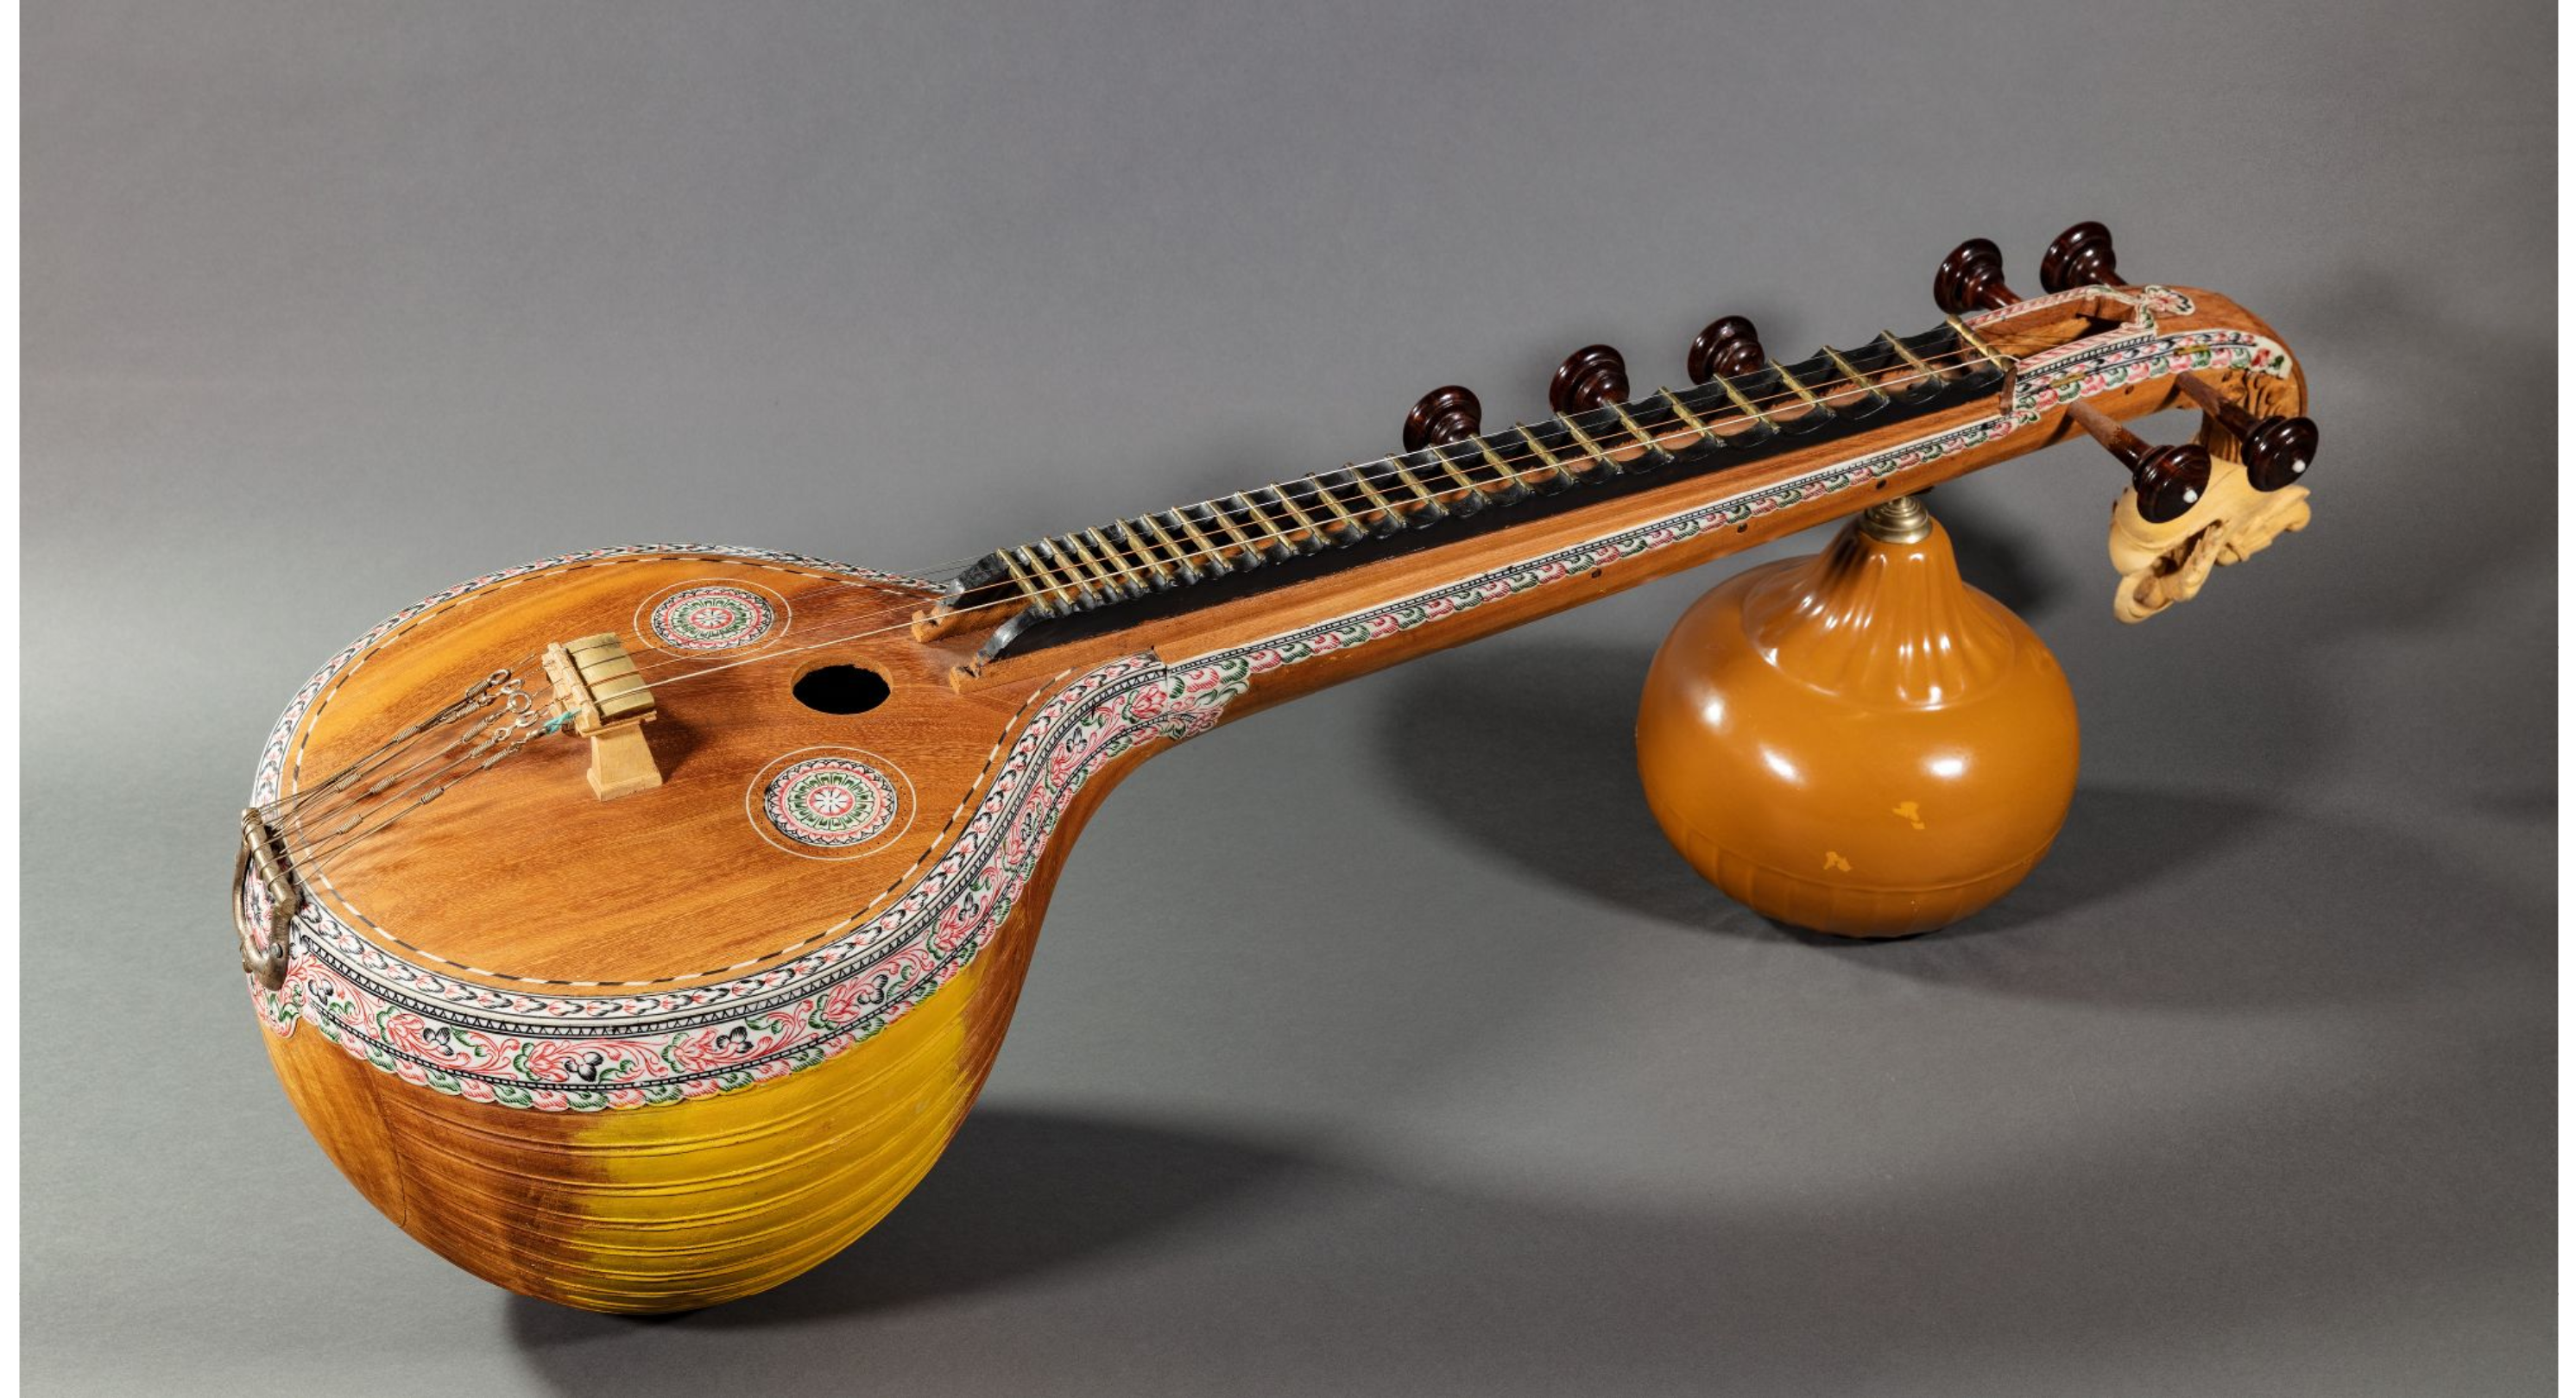
\includegraphics{veena}
  \caption{Veena from Chennai, Wikimedia Commons}
\end{marginfigure}
\begin{marginfigure}[-6\baselineskip]
  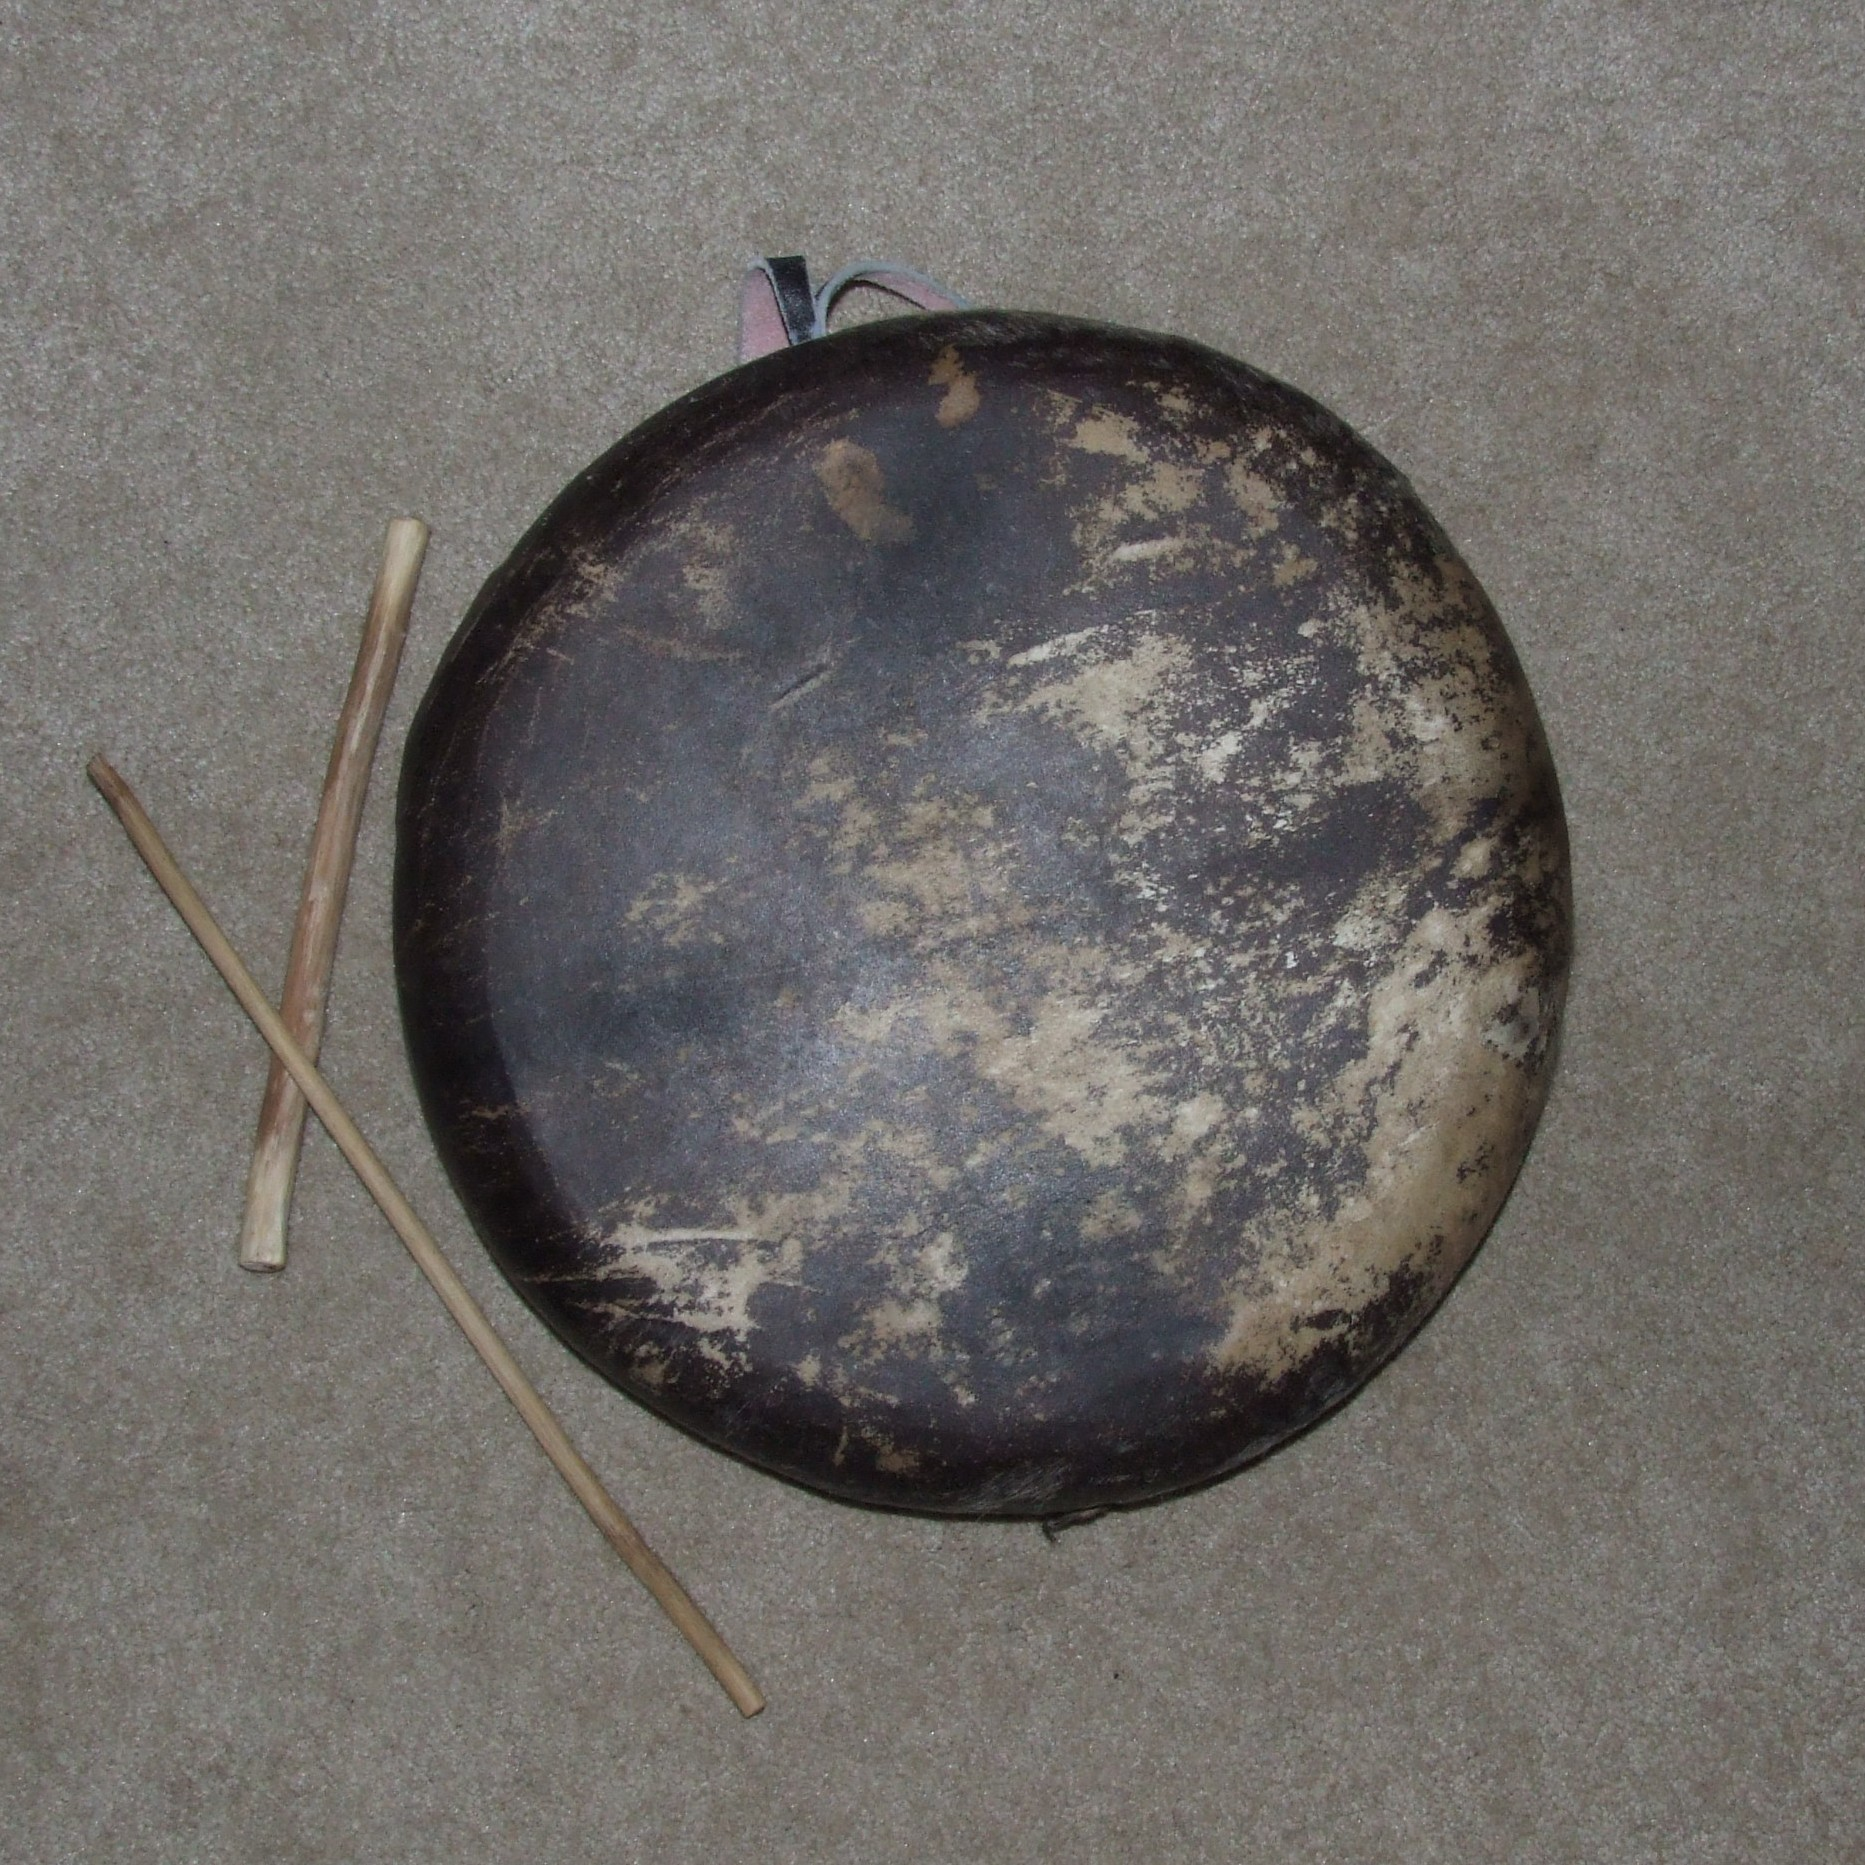
\includegraphics{parai}
\caption{Front side of a parai with the sticks used to play the instrument. Image by Prabhunkl, licensed under CC BY-SA 4.0}  
\end{marginfigure}
\begin{marginfigure}
  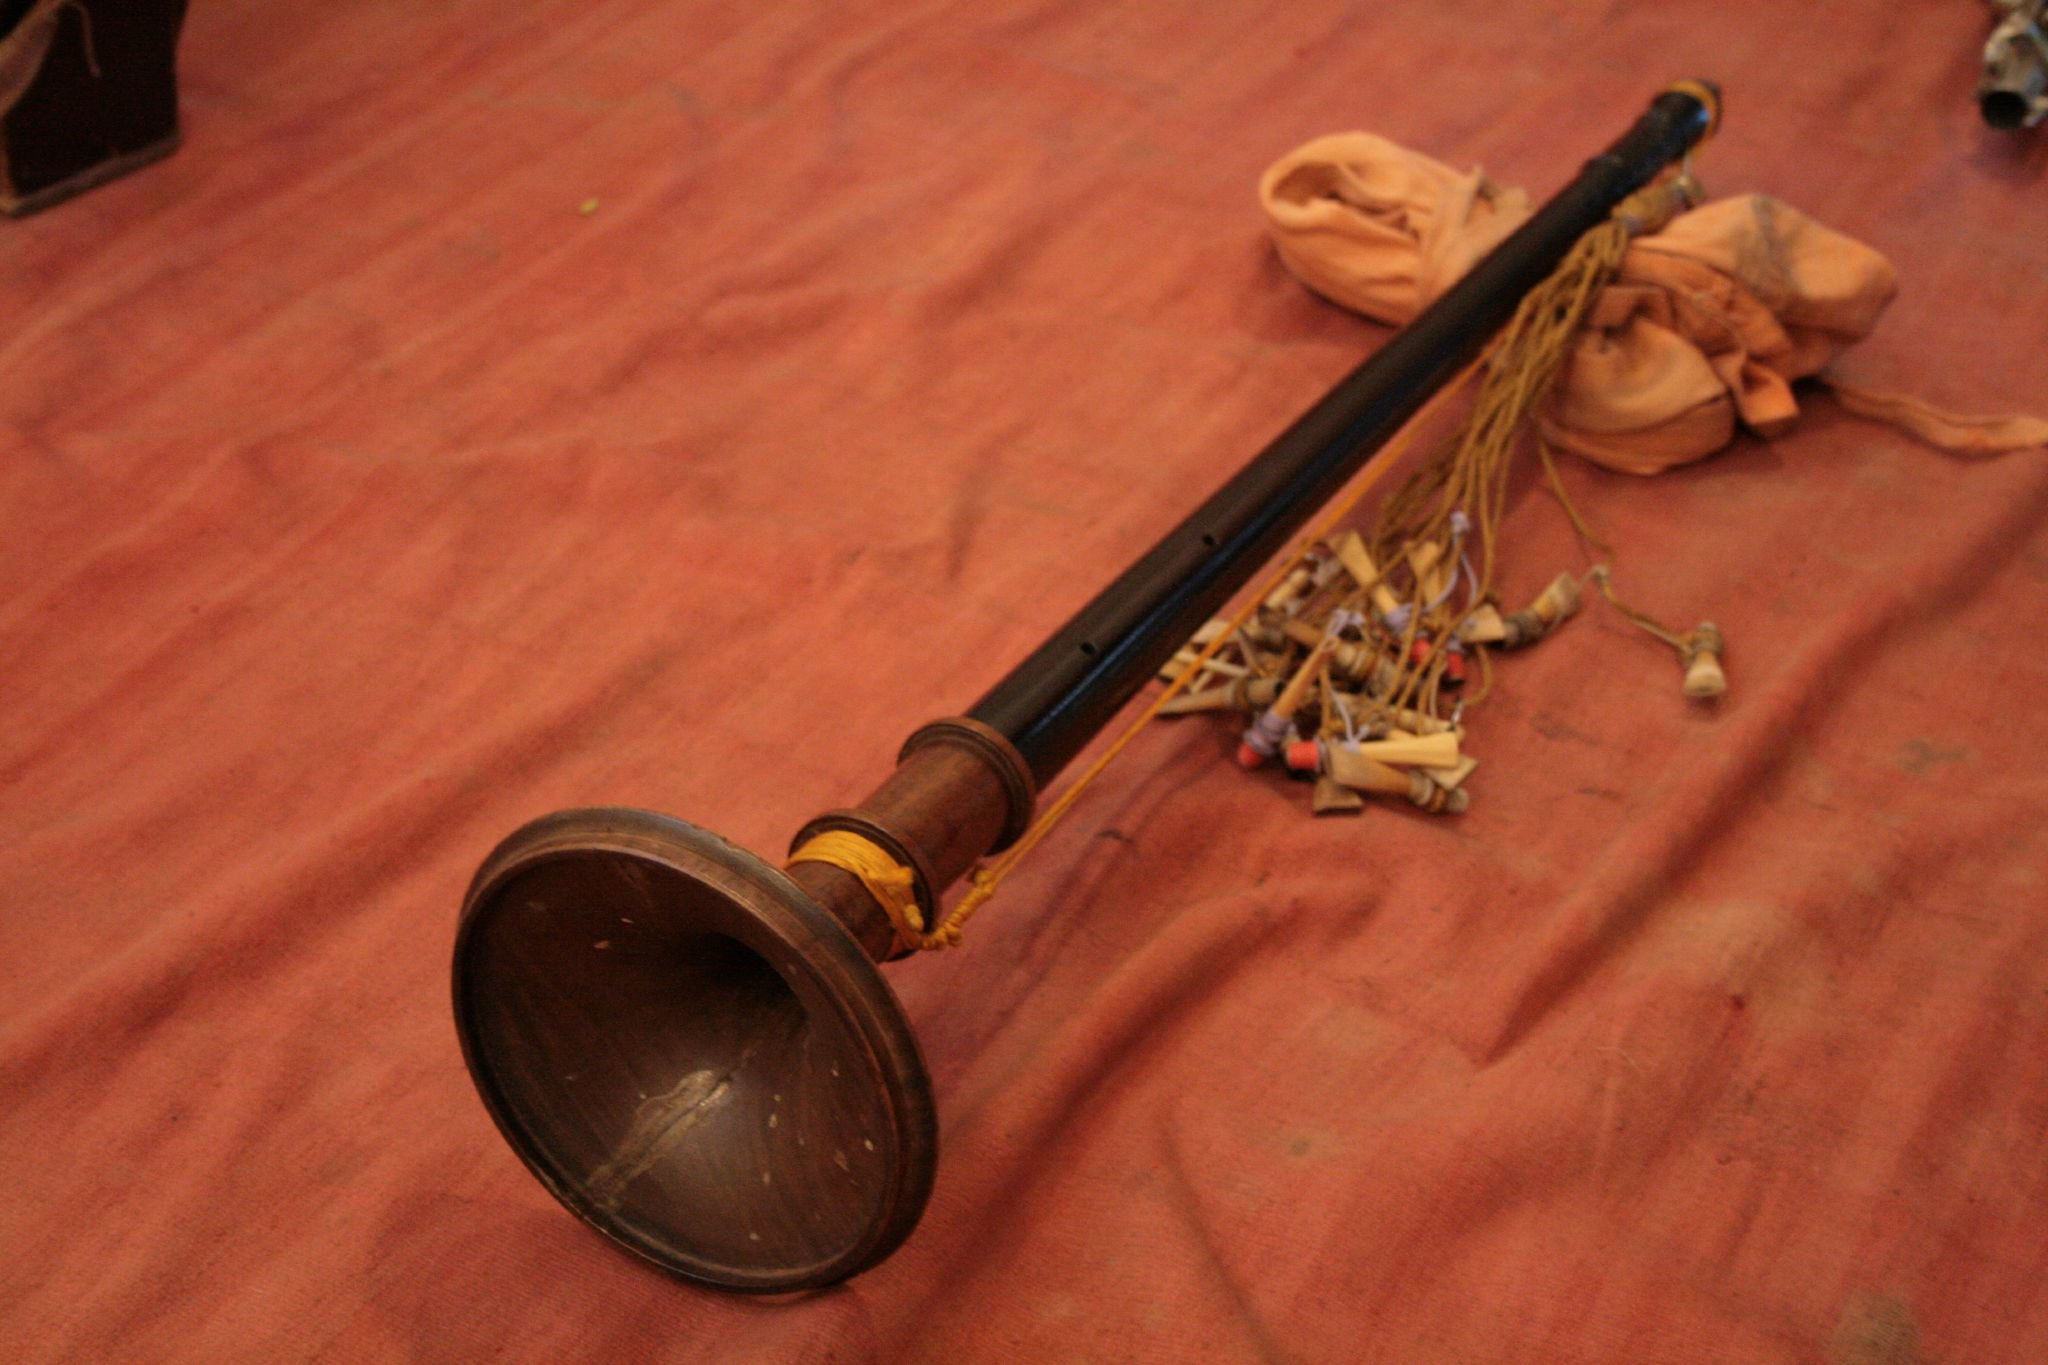
\includegraphics{nadaswaram}
\caption{Nadaswaram (also nagaswaram or nagasuram), Image by Ashwin Kamath}
\end{marginfigure}
\section{How do we produce sound?}
Our voice is also produced by vibrations.

\section{Activity: Feeling the Vibrations in Your Throat}
\subsection{Procedure}
Place your fingers gently on the front of your throat. Say ``Aaa..." loudly for a few seconds. Repeat the activity while whispering ``Aaa...". Compare what you feel in both cases.

\newthought{Observe} Do you feel vibrations in your throat when you speak? Do you feel the same vibrations when you whisper?

\newthought{Discussion} Inside your throat is a small organ called the voice box or larynx. It contains two small muscular bands called vocal cords.
\begin{marginfigure}
  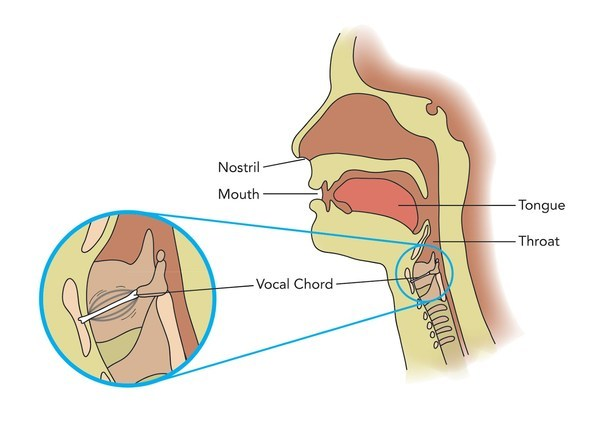
\includegraphics{vocalcord}
  \caption{Our vocal chords vibrate when we produce sound. Image source: SASOL Inzalo Foundation}
\end{marginfigure}
When you breathe, air passes freely through the voice box. When you speak or sing, the vocal cords come close together. Air from the lungs passes between them and makes them vibrate rapidly. These vibrations produce sound.

When you whisper, the vocal cords do not vibrate in the same way. That is why you do not feel the same vibrations in your throat.

\subsection{How Do We Form Different Sounds?}

The sound produced by the vocal cords is only a basic buzzing sound. This sound is shaped into speech by different parts of our mouth. Our tongue, lips, teeth, the roof of the mouth (palate), and the nose work together to produce different sounds and words.

\begin{fullwidth}
\begin{table}[h]
  \centering
  \begin{tabular}{ll}
        \toprule
        Letter & How the sound is made with your mouth, nose, and tongue?\\ 
        \midrule
        {\tam ப} (pa) &Close both lips tightly, then open them suddenly\\
        {\tam ம} (ma) & Close both lips. Let the sound come out through your nose\\
        {\tam த} (tha)& Touch the tip of your tongue to your upper front teeth.\\
        {\tam ல} (la) & Touch the tip of your tongue to the bumpy part just behind your upper front teeth.\\
        {\tam ள} (la) & Curl the tip of your tongue slightly backwards and touch the roof of your mouth.\\
        {\tam ழ} (zha) & Curl the tip of your tongue slightly backwards, but do not let it touch the roof of your mouth.\\
        \bottomrule
  \end{tabular}
\end{table}
\end{fullwidth}

\section{How Does Sound Propagate?}
We have seen that a vibrating object produces sound. But how does the sound reach our ears? When an object vibrates, it pushes and pulls the particles around it. These particles push and pull the particles next to them. In this way, the disturbance moves through the material. For example, when you pluck a rubber band, the rubber band vibrates. It pushes and pulls the air around it. The disturbance then passes from one air particle to the next. When the disturbance reaches the air near your eardrum, your eardrum vibrates and you hear the sound.

The particles of air do not travel all the way from the rubber band to your ear. Instead, they pass the disturbance from one particle to the next. What happens if there are no particles around a vibrating object? A region with no matter is called a vacuum. Sound needs matter to carry its vibrations from one place to another. Therefore, sound cannot travel through a vacuum.

There is almost no atmosphere on the Moon. If two astronauts stand a short distance apart on the Moon and one of them shouts, the other cannot hear the sound directly. Because of this, astronauts on the Moon use radios to communicate with each other.

\begin{marginfigure}[-10\baselineskip]
  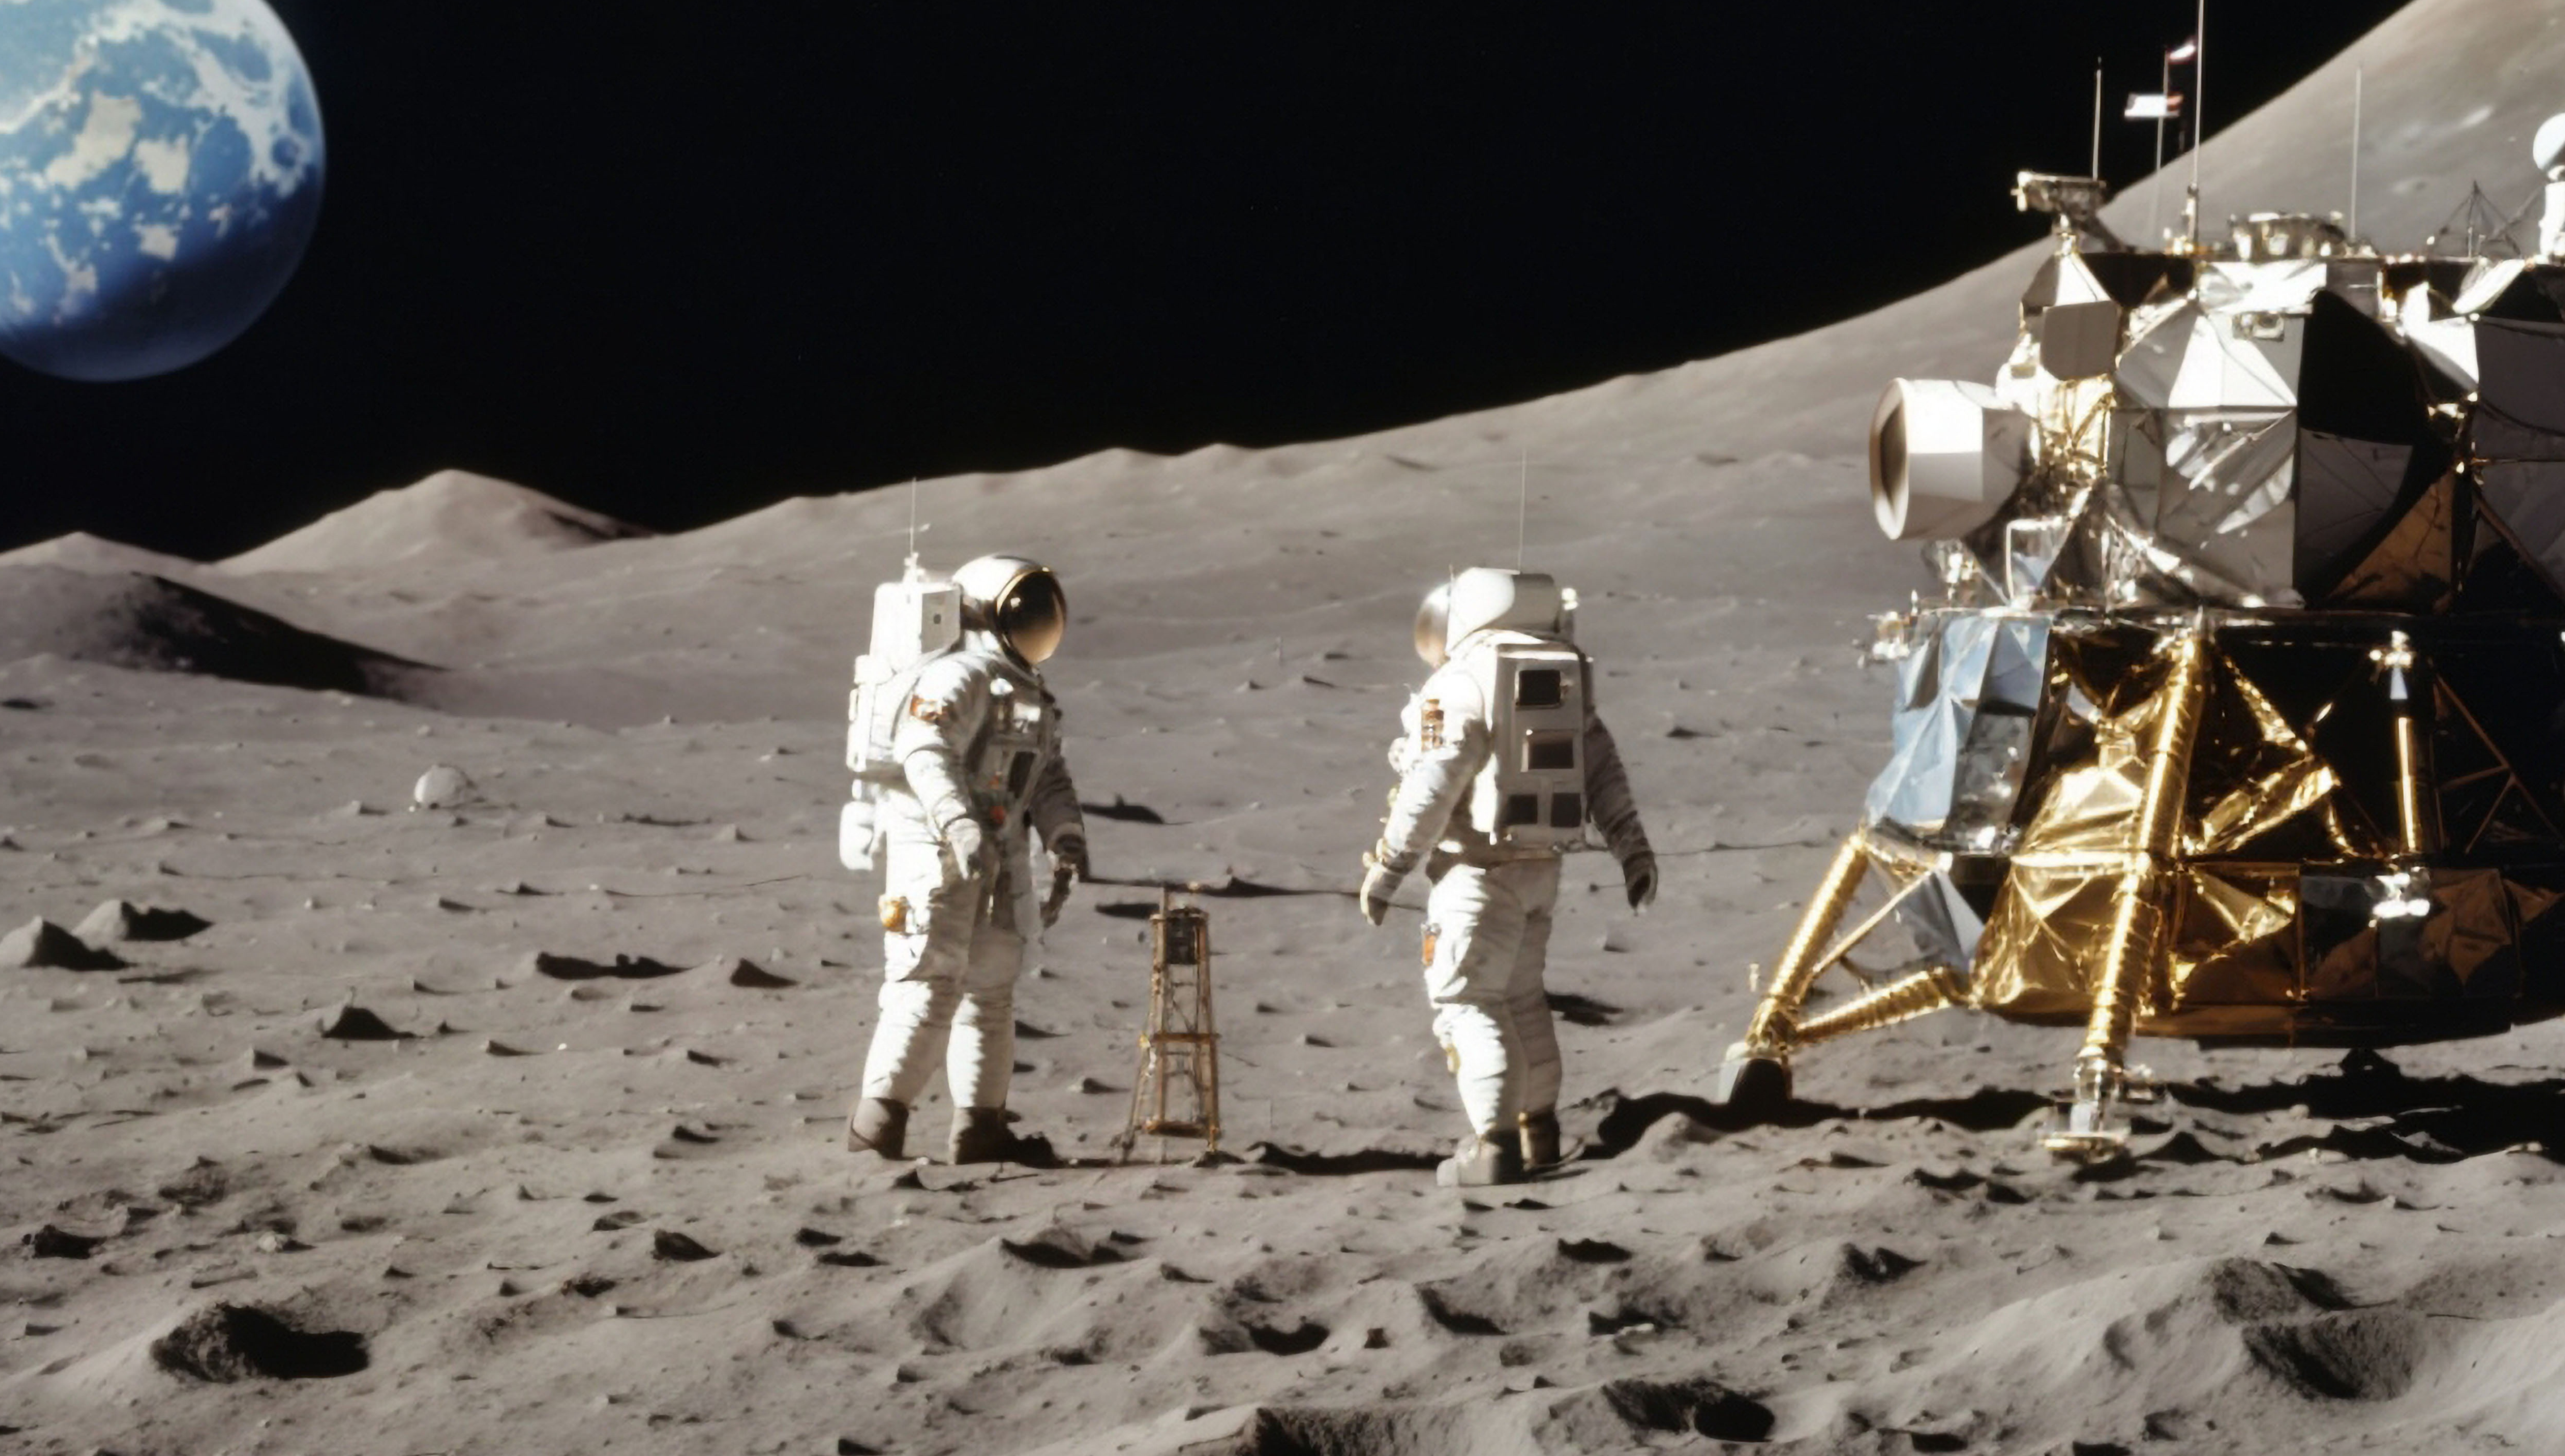
\includegraphics{astronauts}
  \caption{Astronauts on the Moon}
\end{marginfigure}

\marginnote{Did you know? Radios use \textbf{electromagnetic waves}. Electromagnetic waves can travel through empty space.}
\section{Activity: Listening Through Solids}
\subsection{Procedure}
Place your ear on the surface of a desk. Ask your benchmate to tap the desk gently with a pencil a short distance away. Listen carefully to the sound. Lift your ear away from the desk. Ask your benchmate to tap the same place again. Listen to the sound through the air. Compare the two sounds.
\newthought{Observe:} Which sound is louder or clearer? Which path did the sound take: through the desk or through the air?
\newthought{Discussion:} You can hear the sound through the desk. This shows that sound can travel through a solid.

Sound can travel through solids, liquids, and gases. A material through which sound travels is called a medium.
\subsection{Activity: String Telephone}
Materials required:
\begin{enumerate}
\item Two paper cups
\item A long piece of string
\end{enumerate}
Make a small hole at the bottom of each cup. Tie the ends of the string to the cups through these holes. Give one cup to your benchmate. Stand away from your benchmate to keep the string tight. Speak into one cup while your benchmate listens through the other cup. See Figure~\ref{stringtelephone}. Repeat the activity keeping the string loose. Compare the two sounds. 
\begin{figure}[h]
  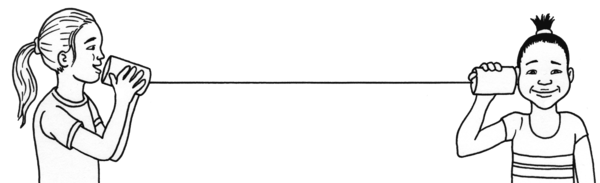
\includegraphics{stringtelephone}
  \caption{Image source: SASOL Inzalo Foundation}
  \label{fig:stringtelephone}
\end{figure}
\newthought{Observe:} Can your benchmate hear your voice when the string is tight? What happens to the sound when you loosen the string?

\newthought{Discuss:} When the string is tight, vibrations travel through the string from one cup to the other. When the string is loose, the vibrations do not travel as well. This activity shows that sound can travel through a solid medium.

\newthought{Question:} Why can astronauts not hear each other directly on the Moon?
\section{Activity: Does Air Travel with Sound?}
\subsection{Materials required}
\begin{enumerate}
    \item A small piece of tissue paper
    \item A sound-producing object, such as a bell or a plate and spoon
\end{enumerate}
\subsection{Procedure}
Hold the piece of tissue paper about 20 to 30 cm away from the sound source. Produce a sound using the bell, or tap the plate gently with a spoon. Watch the tissue paper carefully. Repeat the activity with the tissue paper at different distances from the sound source. Observe the movement of the tissue paper.

\newthought{Observe:} Does the tissue paper move? Does it move as if air is flowing from the sound source towards it? How is this different from the movement of the tissue when you blow air towards it?

\newthought{Discuss:} When you blow air towards the tissue, air flows from your mouth to the tissue and makes it move. When you produce a sound, you do not see air flowing from the sound source towards the tissue in the same way. Instead, the air particles near the sound source move back and forth. They push and pull the particles next to them. The disturbance passes from one particle to the next and eventually reaches our ears. The air particles do not travel all the way from the sound source to our ears. They mainly move back and forth around their usual positions.

When you hear a sound, it is the disturbance, or vibration, that travels from the source to your ear. The air itself does not travel all the way from the source to your ear.

\section{Sound Waves}
We have seen that sound is produced by vibrations. But how does this vibration travel from the source to our ears?

\section{Activity: Long Spring}
\subsection{Materials required}
\begin{enumerate}
\item A long spring or slinky
\item A small ribbon
\end{enumerate}
\begin{marginfigure}
  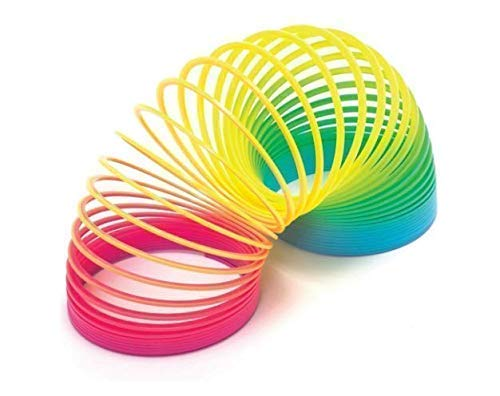
\includegraphics{slinky}
  \caption{Long spring also known as a slinky.}
\end{marginfigure}
\subsection{Procedure}
Hold one end of the spring while your classmate holds the other end. Stretch the spring gently between you. Tie a small ribbon to a single coil near the middle of the spring. Now give the spring a quick push and then pull it backward quickly along the length of the spring. Watch the ribbon carefully.
\begin{marginfigure}
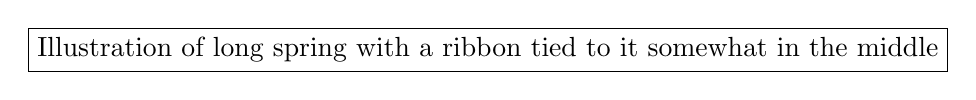
\begin{tikzpicture}
  \node[draw] at (0,0) {Illustration of long spring with a ribbon tied to it somewhat in the middle};
\end{tikzpicture}
  \caption{Illustration of long spring with a ribbon tied to it somewhat in the middle}
\end{marginfigure}

\newthought{Observe:} How does the ribbon move? Does the ribbon travel from one end of the spring to the other? In which direction does the ribbon move?

\newthought{Discussion:} You will notice that the ribbon moves back and forth around its original position. However, the tied ribbon does not travel along the spring. Instead, it moves back and forth around its original resting position. 

The ribbon shows how particles behave in a medium when sound propagates. The medium itself does not flow from the source to the listener. Instead, individual particles vibrate back and forth around fixed positions.

% Air behaves in a similar way when sound propagates through it. Air particles move back and forth around their usual positions, while the disturbance travels from the source to our ears. See Figure~\ref{fig:wavefront}.

% \begin{figure}
%   \begin{tikzpicture}
%     \draw[->] (0,0) -- (4,0);
%     \draw[->] (0,0) -- (230:4);
%     \foreach \i in {2,...,7}{
%       \draw[red,very thick] (0,0) circle [radius=0.5*\i];
%       \draw[red!45, thick] (0,0) circle [radius={0.5*\i+0.1}];
%       \draw[red!45, thick] (0,0) circle [radius={0.5*\i+0.4}];
%       \draw[red!15] (0,0) circle [radius={0.5*\i+0.25}];
%     }
%     \node at (0,0) {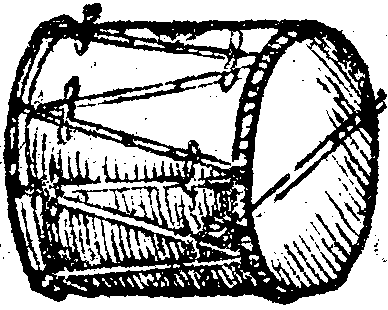
\includegraphics[width=1.25cm]{drum}};
%     \node at (70:3) {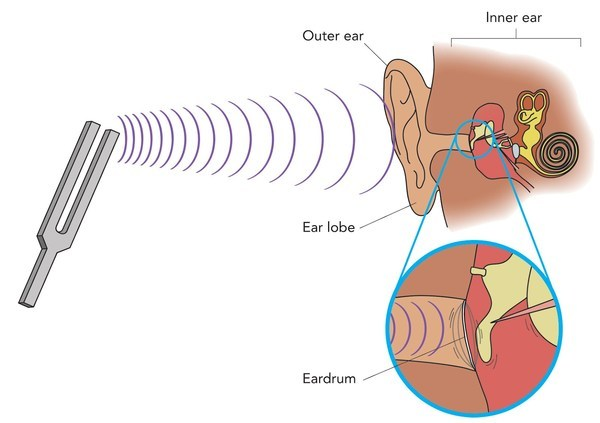
\includegraphics[height=0.8cm]{ear}};
%   \end{tikzpicture}
%   \caption{Sound wave propagates from the source of sound (drum in this case) to the listener in the form of vibrations in the medium.}
%   \label{fig:wavefront}
% \end{figure}

Consider a plucked string. As the vibrating string moves forward, it pushes the nearby air particles together. These particles collide with those in front of them, creating a region of high particle density and high pressure. See Figure~\ref{fig:vibrating-string-to}.
\begin{figure}[h]
  \begin{tikzpicture}
    \node at (0,0) {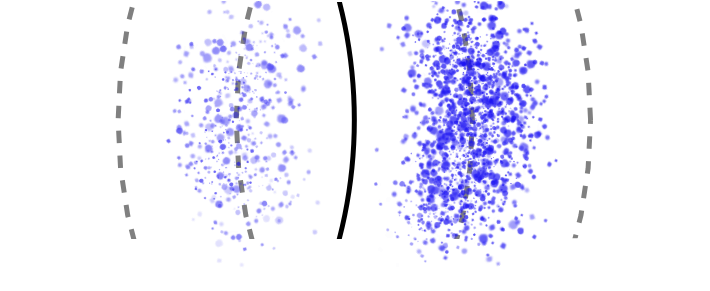
\includegraphics{vibrating-string-to}};
    \draw (0,-2.5) node {String};
    \node at (1.5,2.75) {High pressure and density (Compression)};
    \draw[|-|] (0,2.5) -- (3,2.5);
  \end{tikzpicture}
  \caption{\label{fig:vibrating-string-to}Compression is the region where the air particles are closely packed.}
\end{figure}

When the string springs back, it leaves a region behind it with fewer particles, creating a region of low particle density and low pressure. See Figure~\ref{fig:vibrating-string-fro}.
\begin{figure}[h]
  \begin{tikzpicture}
    \node at (0,0) {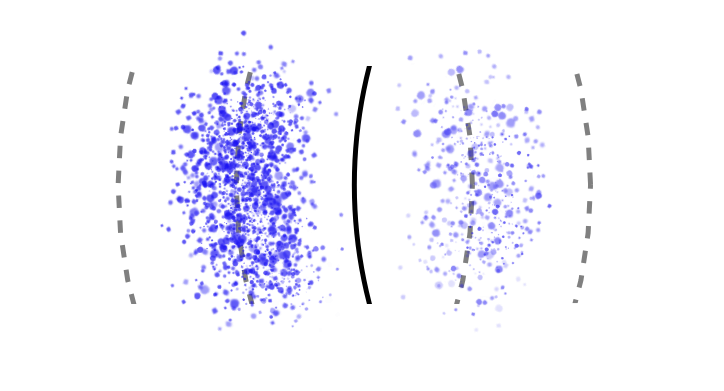
\includegraphics{vibrating-string-fro}};
    \node at (1.5,2.75) {Low pressure and density (Rarefaction)};
    \draw[|-|] (0,2.5) -- (3,2.5);
    \node at (-1.5,-2.75) {Compression};
    \draw[|-|] (-3,-2.5) -- (0,-2.5);
  \end{tikzpicture}
  \caption{\label{fig:vibrating-string-fro}Rarefaction is the region where the air particles are farther apart or loosely packed.}
\end{figure}

After some time, the particles that moved forward now move backward. At that time, the same area where density was high earlier now becomes low in density. Just like the plucked string moves back and forth, the air particles also move back and forth. But only the vibration that was first created keeps travelling forward like a wave. See Figure~\ref{fig:compressionRarefaction}.

\begin{figure}[h]
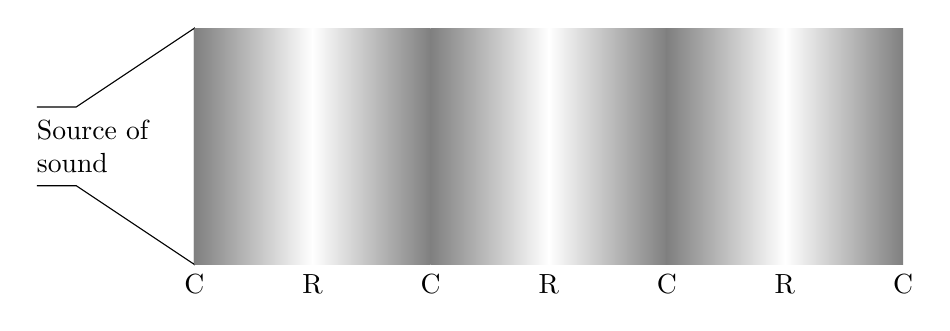
\begin{tikzpicture}
        \pic at (0,0) {speaker};
        \pgfmathsetmacro{\w}{3}
        \foreach \i in {1,2,3}{
          \shadedraw[shading=axis,shading angle=90,draw=none] ({1+(\i-1)*\w},-2) rectangle ({1+(\i-1)*\w+\w/2},{-2+\w});
          \shadedraw[shading=axis,shading angle=-90,draw=none] ({1+(\i-1)*\w+\w/2},-2) rectangle ({1+\i*\w},{-2+\w});
          \node[below] at ({1+(\i-1)*\w},-2) {C};
          \node[below] at ({1+(\i-1)*\w+\w/2},-2) {R};
          }
          \node[below] at ({1+3*\w},-2) {C};
    \end{tikzpicture}
%  \checkparity This is an \pageparity\ page.%
  \caption{\label{fig:compressionRarefaction}Sound propagates as density variations in the medium. C: Compression, R: Rarefaction}
%   \zsavepos{pos:ppfig1}
  \setfloatalignment{b}
\end{figure}

Therefore, to understand sound easily, we picture it as a wave. The part where the wave rises high represents the compression (tight packing) of air. The part where the wave goes low represents the rarefaction (loose packing) of air particles.

\begin{figure}[h]
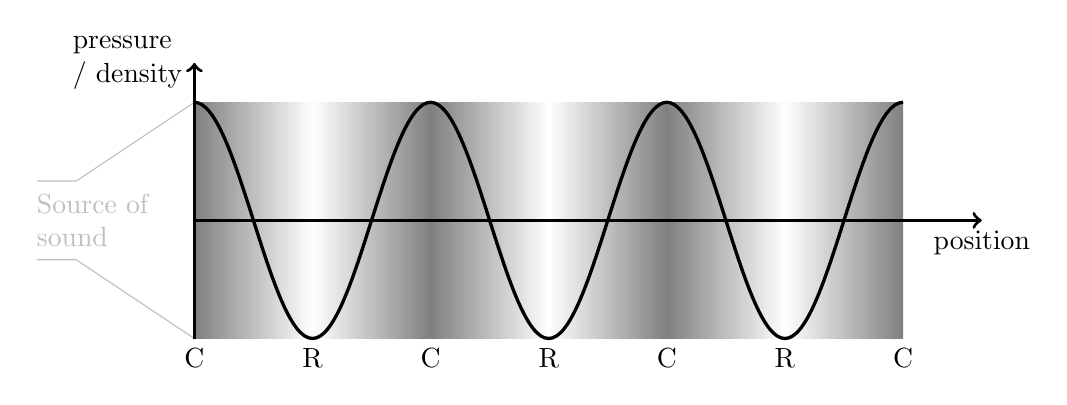
\begin{tikzpicture}
        \pic[gray!50] at (0,0) {speaker};
        \pgfmathsetmacro{\w}{3}
        \pgfmathsetmacro{\d}{0}
        \foreach \i in {1,2,3}{
          \shadedraw[shading=axis,shading angle=90,draw=none] ({1+(\i-1)*\w},-2) rectangle ({1+(\i-1)*\w+\w/2},{-2+\w});
          \shadedraw[shading=axis,shading angle=-90,draw=none] ({1+(\i-1)*\w+\w/2},-2) rectangle ({1+\i*\w},{-2+\w});
          \node[below] at ({1+(\i-1)*\w},-2) {C};
          \node[below] at ({1+(\i-1)*\w+\w/2},-2) {R};
          }
          \node[below] at ({1+3*\w},-2) {C};
          \draw[very thick] (1,{1+\d}) cos (1.75,{-.5+\d}) sin (2.5,{-2+\d}) cos (3.25,{-.5+\d}) sin (4,{1+\d}) cos (4.75,{-.5+\d}) sin (5.5,{-2+\d}) cos (6.25,{-.5+\d}) sin (7,{1+\d}) cos (7.75,{-.5+\d}) sin (8.5,{-2+\d}) cos (9.25,{-.5+\d}) sin (10,{1+\d});
          \draw[very thick,->] (1,{-.5+\d}) -- (11,{-.5+\d}) node[below] {position};
          \draw[very thick,->] (1,{-2+\d}) -- (1,{1.5+\d}) node[left,text width=4em] {pressure / density};
    \end{tikzpicture}
%  \checkparity This is an \pageparity\ page.%
  \caption{The pressure/density variations in the medium vs. position graph for a sound wave.}
  \label{fig:compressionRarefaction-wave}
%   \zsavepos{pos:ppfig1}
  \setfloatalignment{b}
\end{figure}

Look again at the spring activity. The ribbon moves back and forth in the same direction in which the disturbance travels along the spring. Waves in which the particles of the medium move back and forth parallel to the direction of wave travel are called longitudinal waves. Sound waves are longitudinal.

\begin{figure}[h]
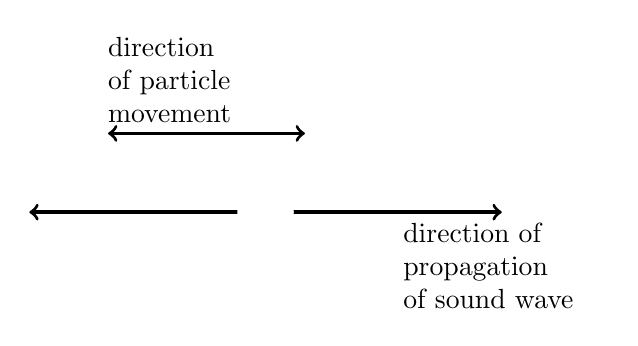
\begin{tikzpicture}
        \pgfmathsetmacro{\w}{3}
        \pgfmathsetmacro{\d}{0}
        \draw[<->,very thick] (0,0) -- (6,0) node[below,text width=2.5cm] {direction of propagation of sound wave};
        \filldraw[white] (3,0) circle [radius=1em];
        \draw[very thick,yshift=1cm,<->] (1,0) -- (3.5,0) node[midway,above,text width=2.5cm] {direction of particle movement};
    \end{tikzpicture}
%  \checkparity This is an \pageparity\ page.%
  \caption{In longitudinal waves, the particles of the medium move parallel to the direction in which the wave propagates.}
  \label{fig:longitudinal-wave}
%   \zsavepos{pos:ppfig1}
  \setfloatalignment{b}
\end{figure}

There is another way in which particles can move in a wave. In ocean waves, water appears to physically move up and then fall down. These waves of sea water consist of alternating crests and troughs that represent high and low points. A crest is the highest point or peak, representing maximum positive displacement, while a trough is the lowest point or valley, representing maximum negative displacement. In this case, the particles move perpendicular to the direction in which the wave travels. Such waves are called \textbf{transverse} waves.

\begin{fullwidth}
\begin{figure}[h]
  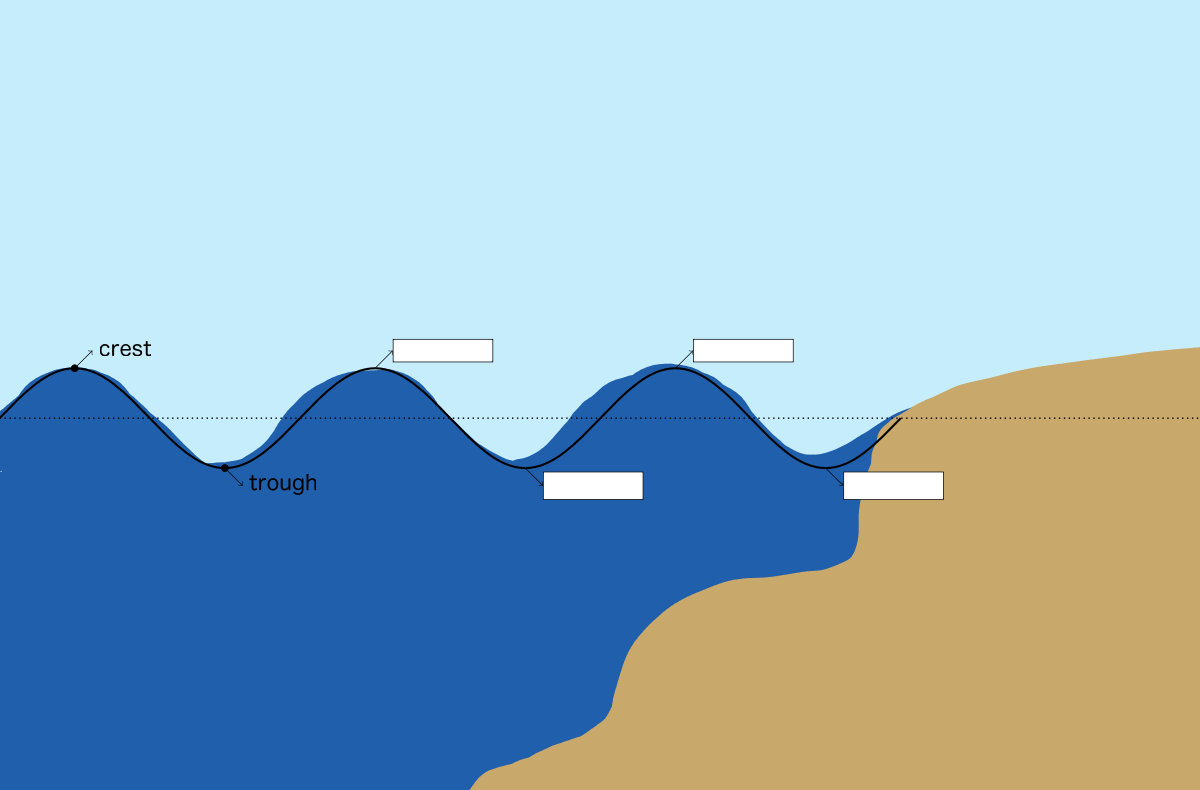
\includegraphics{transverse-wave}
\caption{\label{transverse-wave}In ocean waves, water appears to physically move up and down, forming alternating crests (peaks of positive displacement) and troughs (valleys of negative displacement).}
\end{figure}
\end{fullwidth}

\newthought{Exercise:} Look at the wave diagram in Figure~\ref{transverse-wave}, it shows a snapshot of an ocean weave. Mark and label the crests and troughs.

\begin{figure}[h]
  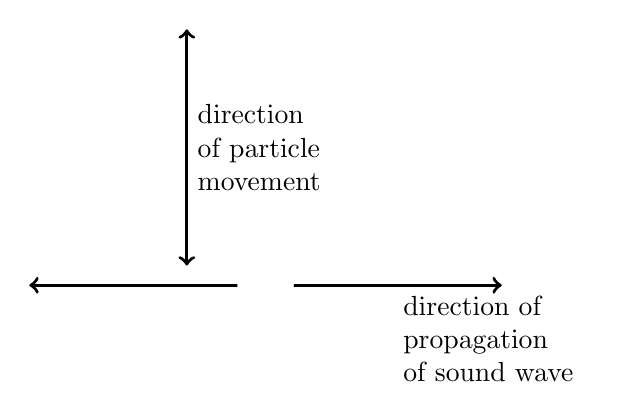
\begin{tikzpicture}
        \pgfmathsetmacro{\w}{3}
        \pgfmathsetmacro{\d}{0}
        \draw[<->,very thick] (0,0) -- (6,0) node[below,text width=2.5cm] {direction of propagation of sound wave};
        \filldraw[white] (3,0) circle [radius=1em];
        \draw[very thick,yshift=0.25cm,<->] (2,0) -- (2,3) node[midway,right,text width=2.5cm] {direction of particle movement};
    \end{tikzpicture}
\caption{In transverse waves, the particles of the medium move perpendicular to the direction in which the wave propagates.}
\end{figure}

A sound wave in air does not have crests and troughs like the ocean wave we see in Figure~\ref{transverse-wave}. The wavy line used to represent how the sound wave changes is only a representation. The actual sound wave consists of particles moving back and forth and regions of compression and rarefaction travelling through the medium. 

\section{Frequency of Sound}

Repeat the Vibrating scale activity. \newthought{Observe:} How does the sound change when the length of the overhanging part changes? Does the scale vibrate faster or slower?

You may notice that when the scale is longer, it vibrates more slowly and the sound is lower. When the scale is shorter, it vibrates faster and the sound is higher. 

\newthought{Discussion:} the number of vibrations that occur in one second is called the \textbf{frequency} of the vibration. Frequency is measured in hertz (\hertz) and usually represented by the Greek letter $\nu$ (nu). Frequency tells us how often an event occurs in a unit of time. Graphically representing sound as a wave helps us understand many of its properties. See Figure~\ref{fig:frequency}.

\newthought{Example:} if you beat a drum 10 times in one second, the frequency of your beating is 10 \hertz.

\begin{figure}[h]
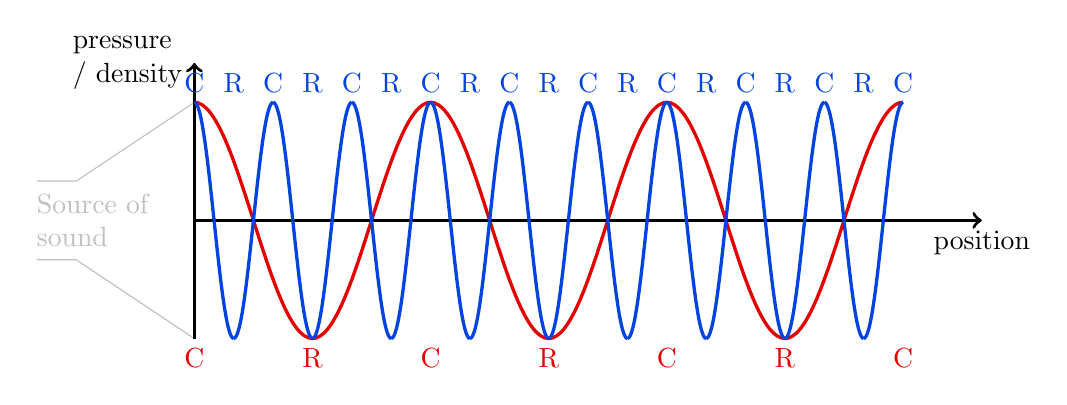
\begin{tikzpicture}
        \pic[gray!50] at (0,0) {speaker};
        \pgfmathsetmacro{\w}{3}
        \pgfmathsetmacro{\d}{0}
        \pgfmathsetmacro{\f}{0.25}
        \foreach \i in {1,2,3}{
          \node[below,xkcdRed] at ({1+(\i-1)*\w},-2) {C};
          \node[below,xkcdRed] at ({1+(\i-1)*\w+\w/2},-2) {R};
          }
          \node[below,xkcdRed] at ({1+3*\w},-2) {C};
          \draw[very thick,xkcdRed] (1,{1+\d}) cos (1.75,{-.5+\d}) sin (2.5,{-2+\d}) cos (3.25,{-.5+\d}) sin (4,{1+\d}) cos (4.75,{-.5+\d}) sin (5.5,{-2+\d}) cos (6.25,{-.5+\d}) sin (7,{1+\d}) cos (7.75,{-.5+\d}) sin (8.5,{-2+\d}) cos (9.25,{-.5+\d}) sin (10,{1+\d});
          \draw[very thick,->] (1,{-.5+\d}) -- (11,{-.5+\d}) node[below] {position};
          \draw[very thick,->] (1,{-2+\d}) -- (1,{1.5+\d}) node[left,text width=4em] {pressure / density};
          \foreach \m in {1,5,9,...,33}{
          \draw[very thick,xkcdBlue] ({1+(\m-1)*\f},{1+\d}) cos ({1+\m*\f},{-.5+\d}); 
          \draw[very thick,xkcdBlue] ({1+\m*\f},{-.5+\d}) sin ({1+(\m+1)*\f},{-2+\d}); 
          \draw[very thick,xkcdBlue] ({1+(\m+1)*\f},{-2+\d}) cos ({1+(\m+2)*\f},{-.5+\d}); 
          \draw[very thick,xkcdBlue] ({1+(\m+2)*\f},{-.5+\d}) sin ({1+(\m+3)*\f},{1+\d}); 
          }
        \foreach \n in {1,2,3,...,9}{
          \node[xkcdBlue,above] at ({\n*\w/3},1) {C};
          \node[xkcdBlue,above] at ({\n*\w/3+0.5},1) {R};
          }
          \node[xkcdBlue,above] at ({10*\w/3},1) {C};
    \end{tikzpicture}
%  \checkparity This is an \pageparity\ page.%
  \caption{\label{fig:frequency}Figure shows sound of two different frequencies. The sound represented as a blue wave has 9 cycles, while the red wave has 3 cycles in the same time. This means that the blue wave completes 3 times as many vibrations in the same time. Therefore, its frequency is 3 times that of the red wave.}
%   \zsavepos{pos:ppfig1}
  \setfloatalignment{b}
\end{figure}

\newthought{Exercise:} Look at the wave diagram in Figure~22, it shows a sound wave recorded over a time period of 2 seconds. Mark and label the regions of compressions and rarefactions on the diagram.

\begin{figure}[h]
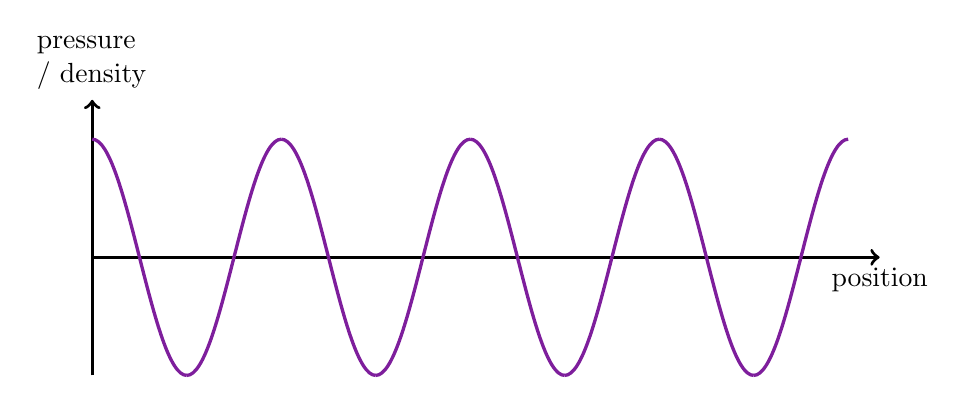
\begin{tikzpicture}
%         \pgfmathsetmacro{\w}{3}
        \pgfmathsetmacro{\d}{0}
        \pgfmathsetmacro{\f}{0.6}
          \draw[very thick,->] (1,{-.5+\d}) -- (11,{-.5+\d}) node[below] {position};
          \draw[very thick,->] (1,{-2+\d}) -- (1,{1.5+\d}) node[above,text width=4em] {pressure / density};
          \foreach \m in {1,5,9,13}{
          \draw[very thick,xkcdPurple] ({1+(\m-1)*\f},{1+\d}) cos ({1+\m*\f},{-.5+\d}); 
          \draw[very thick,xkcdPurple] ({1+\m*\f},{-.5+\d}) sin ({1+(\m+1)*\f},{-2+\d}); 
          \draw[very thick,xkcdPurple] ({1+(\m+1)*\f},{-2+\d}) cos ({1+(\m+2)*\f},{-.5+\d}); 
          \draw[very thick,xkcdPurple] ({1+(\m+2)*\f},{-.5+\d}) sin ({1+(\m+3)*\f},{1+\d}); 
          }
    \end{tikzpicture}
  \caption{Sound wave recorded over a time period of 2 seconds.}\label{fig:frequency-exercise}
  \setfloatalignment{b}
  \end{figure}

  \newthought{Exercise:} Count the total number of complete wave cycles that occur within the 2-second time period shown in the figure. A cycle (or wave cycle) is one complete pattern of a wave. For a sound wave, one single cycle consists of one full compression plus one full rarefaction (or the distance from the start of one compression to the start of the next). It represents one complete back-and-forth vibration.

  \newthought{Exercise:} Use your count from the previou exercise to calculate the frequency of the wave. Frequency is the number of complete cycles per second, measured in Hertz (\hertz).

\section{Pitch}
Sounds with higher frequency have a higher pitch and sounds with lower frequency have a lower pitch. A mosquito makes a high-pitched sound. A drum makes a low-pitched sound. Which one is vibrating faster?

\section{Activity: Singing Pipe and Glass}
\subsection{Materials required}
\begin{enumerate}
  \item A glass, transparent cup, or water bottle
  \item A thin hollow pipe
  \item water
\end{enumerate}
\subsection{Procedure}
Fill the glass about three-quarters full with water. Place the pipe vertically in the water leaving one end of the pipe above the water. Blow gently across the open end of the pipe. Listen to the sound produced. Next, move the pipe up so that a longer part of the pipe is above the water. Blow across the open end again. Move the pipe down so that a shorter part of the pipe is above the water. Blow across the open end again. Compare the sounds.
\begin{figure}
  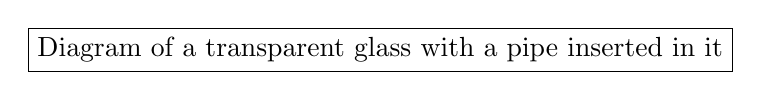
\begin{tikzpicture}
    \node[draw] at (0,0) {Diagram of a transparent glass with a pipe inserted in it};
  \end{tikzpicture}
  \caption{Singing Pipe and Glass}
\end{figure}
\marginnote{Ask your teacher to help you use the \textbf{Phyphox} app on their smartphone to measure the frequency of the sounds. Compare the frequency of the high-pitched and low-pitched sounds.}

\newthought{Observe:} Does the sound change when you change the length of the air column?

\newthought{Discussion:} Changing the length of the air column changes the pitch of the sound.

\newthought{Question:} Which one is vibrating faster? Mosquito's wings or the membrane of the drum?

\subsection{Amplitude}
You may also have noticed something else during the vibrating scale activity. When the scale was plucked gently, the sound was soft. When the scale was plucked harder, the sound was louder. 

If you watch the scale carefully, you will see that when it is plucked harder, it moves farther away from its resting position during each vibration.

The size of this vibration is called the \textbf{amplitude}. Amplitude tells us how large the vibration is. A vibration with greater amplitude produces a louder sound, while a vibration with smaller amplitude produces a softer sound. Amplitude affects loudness, not pitch. The sound level can be measured using a unit called the decibel (dB). In a graphical representation of a sound wave, the amplitude is shown by the distance of the wave from its middle or resting position. A larger amplitude is shown by a taller wave. See Figure~\ref{fig:amplitude}.

\begin{figure}[h]
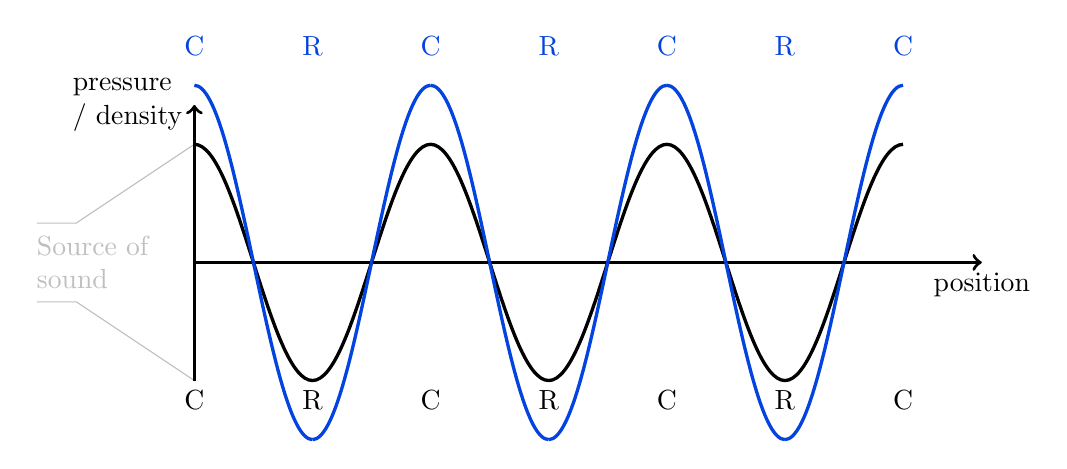
\begin{tikzpicture}
        \pic[gray!50] at (0,0) {speaker};
        \pgfmathsetmacro{\w}{3}
        \pgfmathsetmacro{\d}{0}
        \pgfmathsetmacro{\f}{0.75}
        \foreach \i in {1,2,3}{
          \node[below] at ({1+(\i-1)*\w},-2) {C};
          \node[below] at ({1+(\i-1)*\w+\w/2},-2) {R};
          }
          \node[below] at ({1+3*\w},-2) {C};
          \draw[very thick] (1,{1+\d}) cos (1.75,{-.5+\d}) sin (2.5,{-2+\d}) cos (3.25,{-.5+\d}) sin (4,{1+\d}) cos (4.75,{-.5+\d}) sin (5.5,{-2+\d}) cos (6.25,{-.5+\d}) sin (7,{1+\d}) cos (7.75,{-.5+\d}) sin (8.5,{-2+\d}) cos (9.25,{-.5+\d}) sin (10,{1+\d});
          \draw[very thick,->] (1,{-.5+\d}) -- (11,{-.5+\d}) node[below] {position};
          \draw[very thick,->] (1,{-2+\d}) -- (1,{1.5+\d}) node[left,text width=4em] {pressure / density};
          \foreach \m in {1,5,9}{
          \draw[very thick,xkcdBlue] ({1+(\m-1)*\f},{1.75+\d}) cos ({1+\m*\f},{-.5+\d}); 
          \draw[very thick,xkcdBlue] ({1+\m*\f},{-.5+\d}) sin ({1+(\m+1)*\f},{-2.75+\d}); 
          \draw[very thick,xkcdBlue] ({1+(\m+1)*\f},{-2.75+\d}) cos ({1+(\m+2)*\f},{-.5+\d}); 
          \draw[very thick,xkcdBlue] ({1+(\m+2)*\f},{-.5+\d}) sin ({1+(\m+3)*\f},{1.75+\d}); 
          }
        \foreach \n in {1,2,3}{
          \node[xkcdBlue,above] at ({1+(\n-1)*\w},2) {C};
          \node[xkcdBlue,above] at ({1+(\n-1)*\w+\w/2},2) {R};
          }
          \node[xkcdBlue,above] at ({1+3*\w},2) {C};
    \end{tikzpicture}
%  \checkparity This is an \pageparity\ page.%
  \caption{\label{fig:amplitude}Figure shows sound of two different amplitudes. The sound represented as a blue wave has larger amplitude compared to the black wave.}
%   \zsavepos{pos:ppfig1}
  \setfloatalignment{b}
\end{figure}

\newthought{Question:} Two sounds have the same pitch, but one is louder. What must be different?

\marginnote{Pitch depends on frequency, which is determined by the source. Distance from the source does not change the frequency. As sound spreads out, its amplitude decreases, this is why it becomes quieter as you move far from the source.}

\section{Wavelength}
The distance between two neighbouring compressions (or two neighbouring rarefactions) is called the \textbf{wavelength}. Wavelength is measured in the units of distance. The SI unit of distance is the metre (m). Wavelength is usually represented by the Greek letter $\lambda$ (lambda). In the graphical representation of sound as wave, the distance between two neighbouring compressions (or two neighbouring rarefactions) is the wavelength. See Figure~\ref{fig:wavelength}. 
\begin{figure}[h]
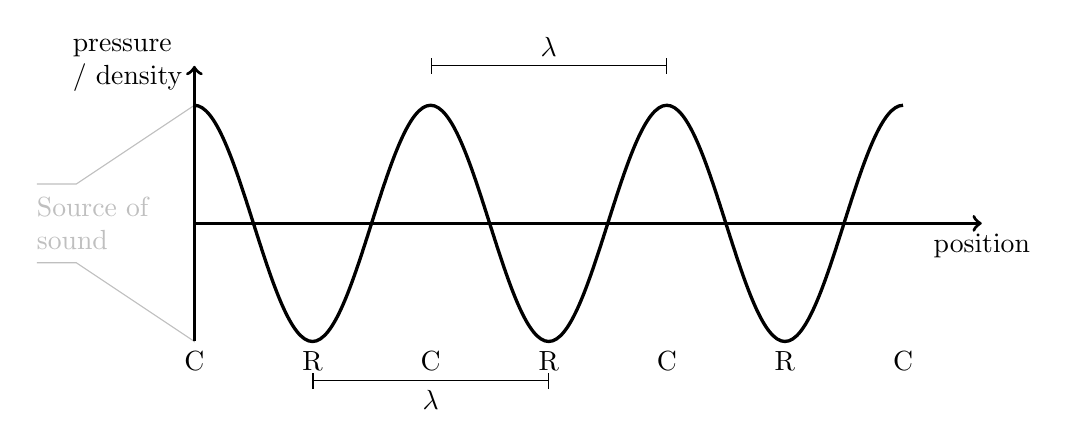
\begin{tikzpicture}
        \pic[gray!50] at (0,0) {speaker};
        \pgfmathsetmacro{\w}{3}
        \pgfmathsetmacro{\d}{0}
        \foreach \i in {1,2,3}{
          \node[below] at ({1+(\i-1)*\w},-2) {C};
          \node[below] at ({1+(\i-1)*\w+\w/2},-2) {R};
          }
          \node[below] at ({1+3*\w},-2) {C};
          \draw[very thick] (1,{1+\d}) cos (1.75,{-.5+\d}) sin (2.5,{-2+\d}) cos (3.25,{-.5+\d}) sin (4,{1+\d}) cos (4.75,{-.5+\d}) sin (5.5,{-2+\d}) cos (6.25,{-.5+\d}) sin (7,{1+\d}) cos (7.75,{-.5+\d}) sin (8.5,{-2+\d}) cos (9.25,{-.5+\d}) sin (10,{1+\d});
          \draw[very thick,->] (1,{-.5+\d}) -- (11,{-.5+\d}) node[below] {position};
          \draw[very thick,->] (1,{-2+\d}) -- (1,{1.5+\d}) node[left,text width=4em] {pressure / density};
          \draw[|-|,yshift=-2.5cm] (2.5,0) -- ++(3,0) node[midway,below] {$\lambda$};
          \draw[|-|,yshift=1.5cm] (4,0) -- ++(3,0) node[midway,above] {$\lambda$};
    \end{tikzpicture}
%  \checkparity This is an \pageparity\ page.%
  \caption{\label{fig:wavelength}The distance between two neighbouring compressions (or two neighbouring rarefactions) is the wavelength ($\lambda$).}
%   \zsavepos{pos:ppfig1}
  \setfloatalignment{b}
\end{figure}

\newthought{Exercise:} In Figure~\ref{fig:exercise-wavelength}, find the wavelength of the sound wave. Give your answer in centimetres (cm).

\begin{figure}
  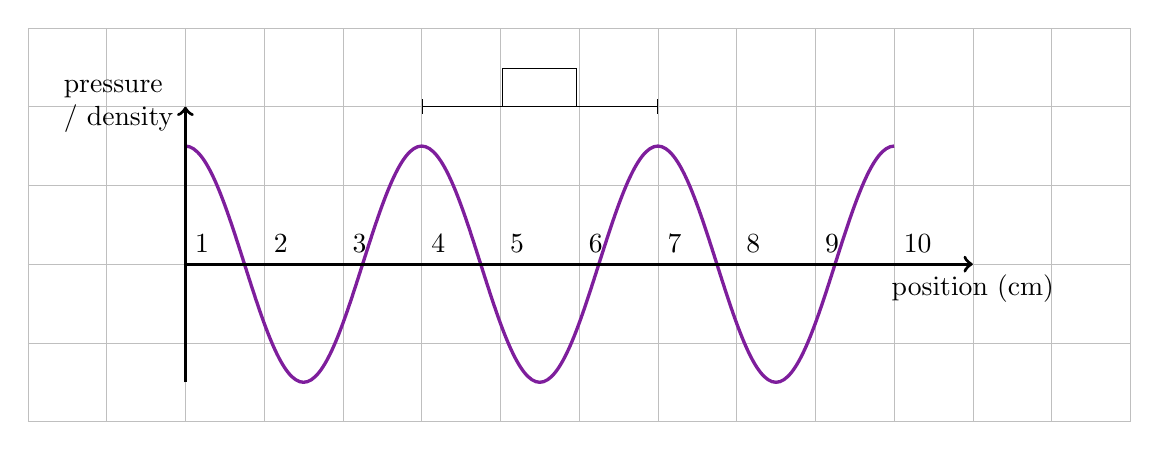
\begin{tikzpicture}
    \draw[yshift=0.5cm,very thin,gray!50] (-1,-3) grid (13,2);
        \pgfmathsetmacro{\w}{3}
        \pgfmathsetmacro{\d}{0}
        \foreach \i in {1,2,3,...,10}{
          \node[below right] at (\i,0) {\i};
        %   \node[below] at ({1+(\i-1)*\w+\w/2},-2) {R};
          }
        %   \node[below] at ({1+3*\w},-2) {C};
          \draw[very thick,xkcdPurple] (1,{1+\d}) cos (1.75,{-.5+\d}) sin (2.5,{-2+\d}) cos (3.25,{-.5+\d}) sin (4,{1+\d}) cos (4.75,{-.5+\d}) sin (5.5,{-2+\d}) cos (6.25,{-.5+\d}) sin (7,{1+\d}) cos (7.75,{-.5+\d}) sin (8.5,{-2+\d}) cos (9.25,{-.5+\d}) sin (10,{1+\d});
          \draw[very thick,->] (1,{-.5+\d}) -- (11,{-.5+\d}) node[below] {position (cm)};
          \draw[very thick,->] (1,{-2+\d}) -- (1,{1.5+\d}) node[left,text width=4em] {pressure / density};
          \draw[|-|,yshift=1.5cm] (4,0) -- ++(3,0) node[midway,above,text=white,fill=white,draw,text width=2em] {$\lambda$};
    \end{tikzpicture}
    \caption{\label{fig:exercise-wavelength}The figure shows how the pressure changes as sound travels through the medium. The horizontal axis shows distance in centimetres (cm).}
\end{figure}

\section{}

Almost all natural sounds (a human voice, falling rain, or a musical instrument) are a complex mixture of multiple sound waves with different frequencies, amplitudes, and wavelengths traveling together through the air. See Figure~\ref{fig:mixedfrequencies}.

\begin{figure}
  \begin{tikzpicture}
    \node[yshift=-4em] at (0,0) {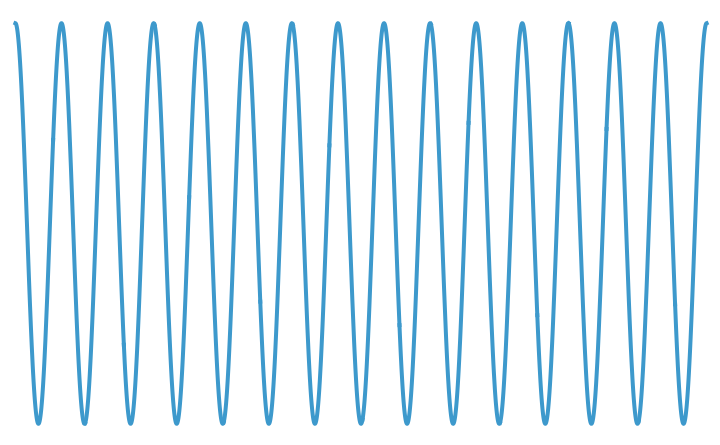
\includegraphics[width=3cm]{cos6x}};
    \node[yshift=-3em] at (0,1) {$+$};
    \node[yshift=-2em] at (0,2) {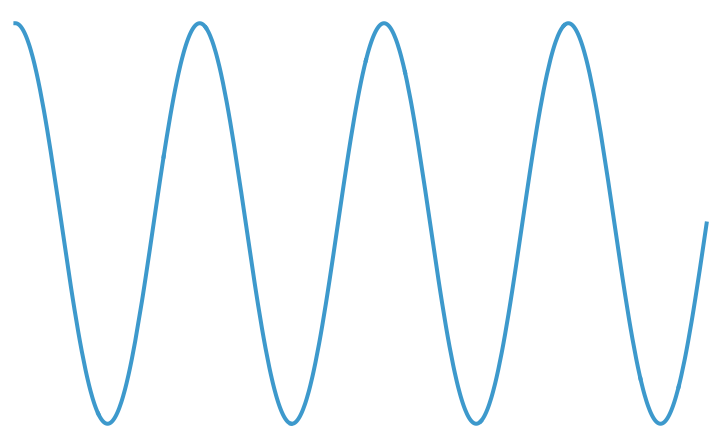
\includegraphics[width=3cm]{3by2Cos3xby2}};
    \node[yshift=-1em] at (0,3) {$+$};
    \node at (0,4) {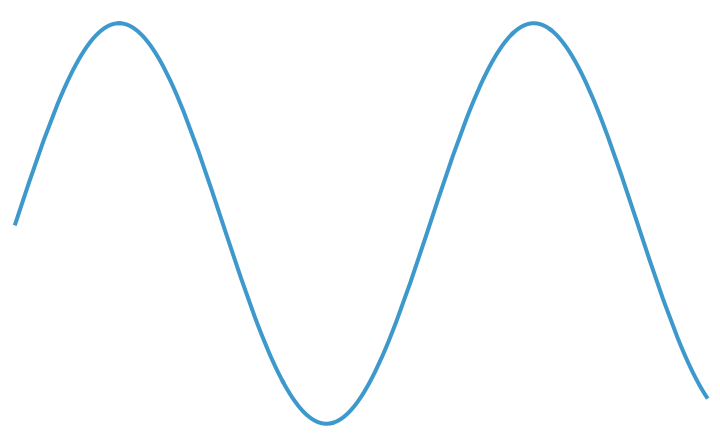
\includegraphics[width=3cm]{2sin2xby3}};
    \node[yshift=1em] at (0,5) {$+$};
    \node[yshift=2em] at (0,6) {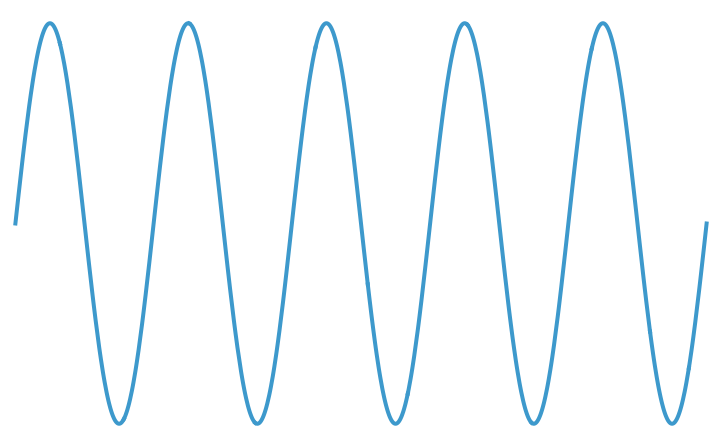
\includegraphics[width=3cm]{sin2x}};
    \node[yshift=3em] at (0,7) {$+$};
    \node[yshift=4em] at (0,8) {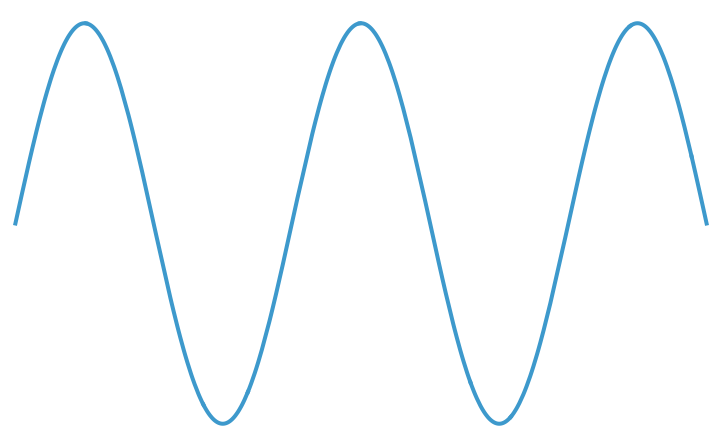
\includegraphics[width=3cm]{sinx}};
    \node at (-2,4) {$=$};
    \node at (-4,4) {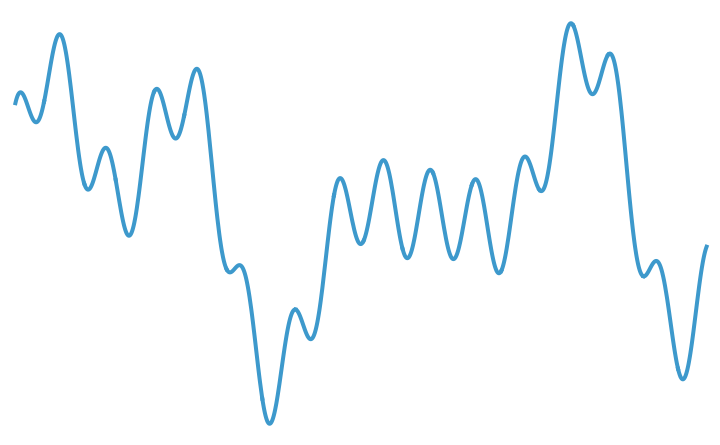
\includegraphics[width=3cm]{total}};
  \end{tikzpicture}
  \caption{\label{fig:mixedfrequencies}The natural sound is a mixture of sound waves with various frequency and wavelengths.}
\end{figure}

Sound systems have different controls that allow us to change the sound we hear. The volume control increases or decreases the amplitude of the sound waves. This makes the sound louder or softer without changing its pitch. The bass control increases or decreases low-frequency sounds, which we hear as deeper sounds, such as the beat of a drum or the sound of a large motor. The treble control increases or decreases high-frequency sounds, which we hear as sharper sounds, such as a whistle, a bell, or the chirping of a bird.
\begin{marginfigure}
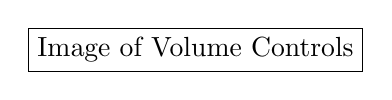
\begin{tikzpicture}
  \node[draw] at (0,0) {Image of Volume Controls};
\end{tikzpicture}
  \caption{Image of Volume Controls on a Sound System}
\end{marginfigure}

\section{}
Unwanted sounds around us, such as the hum of a ceiling fan, the sound of a bus engine, or people talking in a crowded place, are called background noise. Some modern headphones use Active Noise Cancellation (ANC) to reduce background noise. A small microphone in the headphones picks up sounds from the surroundings. The headphones then produce another sound wave that is carefully matched to the unwanted sound. This new wave has the opposite pattern to the unwanted sound wave. When the two waves meet, they partly cancel each other. As a result, the background noise becomes much softer.
\section{}

Repeat the Long Spring activity, but now create compressions more quickly.

\newthought{Observe:} When vibrations happen more often each second (higher frequency), the compressions are packed closer together and the wavelength becomes shorter.

\section{Speed of Sound}
Do we hear sound instantly after it is produced? Think about what happens during lightning and thunder. When lightning strikes, we see a flash of light and hear thunder.

\newthought{Observe:} Do you see the lightning and hear the thunder at the same time? Or do they happen one after the other? Which do you notice first?

Usually, we see the lightning first and hear the thunder later.

\begin{marginfigure}
  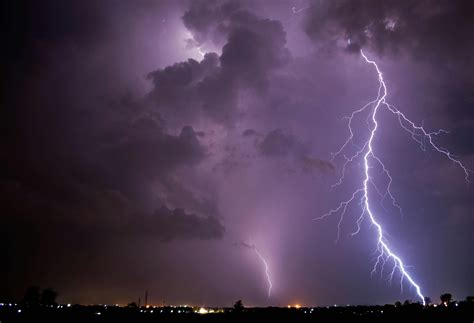
\includegraphics{thunder}
  \caption[Thunder and lightening]{Thunderstorm in Tiruchirappalli, Photo by Amol Mande}
\end{marginfigure}

% \marginnote{If the thunder sounds quieter when you are farther away, does the thunder have less energy when it reaches you?}

These observations show that sound takes time to propagate from the source to our ears. Light travels much faster than sound, so we see the flash before we hear the sound. 

In air, sound propagates at a speed of about 340 metres per second (at room temperature). The speed of a sound wave depends on both its frequency and its wavelength.

\begin{equation}
\text{Speed} = \text{Frequency}\times\text{Wavelength}
\end{equation}

Sound does not propagate at the same speed in all materials. The speed of sound depends on the medium through which it propagates. Sound propagates fastest in solids, slower in liquids, and slowest in gases. For example, sound propagates faster in metal or wood than in air. This is because the particles in solids are closer together, allowing vibrations to pass more quickly from one particle to the next. 

\newthought{Exercise:} A school bell produces a sound with a frequency of 10,000 \hertz. The speed of sound in air is 340 m/s. Calculate the wavelength of the sound wave.

\newthought{Exercise:} The school bell is now completely submerged in water. The bell still vibrates at a frequency of 10 k\hertz. The speed of sound in water is 1500~m/s. Calculate the wavelength of the sound in water.

\marginnote{1~k\hertz = 1000 \hertz.}

\newthought{Discuss:} The frequency of the bell does not change when it is moved from air to water. Does its wavelength change? Explain your answer.

\newthought{Exercise:} A lightning flash is seen instantly, and thunder is heard 4 seconds later. If the speed of sound is 340 m/s, how far away did the lightning strike?

\newthought{Question:} How does temperature affect the speed of sound?

\marginnote{As the temperature increases, the speed of sound increases. This happens because when the temperature is higher, the particles of the medium move faster. As a result, they pass the vibrations to neighbouring particles more quickly, allowing sound to propagate faster. For example, sound travels faster in warm air than in cold air.}

\section{How Do We Hear and Process Sound}
The human ear converts sound waves into electrical signals for the brain. First, the outer part of our ear, called the pinna, collects sound waves and guides them down the ear canal. At the end of this canal, the sound waves strike a thin membrane called the eardrum, making it vibrate like the skin of a drum. The eardrum is connected to three tiny bones inside the ear. These bones are called the malleus, incus, and stapes. These bones amplify the vibrations. The amplified vibrations pass into the cochlea, a snail-shaped tube filled with liquid. As the liquid inside the cochlea ripples, it stimulates tiny hair cells inside the cochlea. These hair cells convert mechanical vibrations into electrical signals. The auditory nerve carries electrical signals to the brain, which interprets them as speech or music.

\begin{figure}[h]
  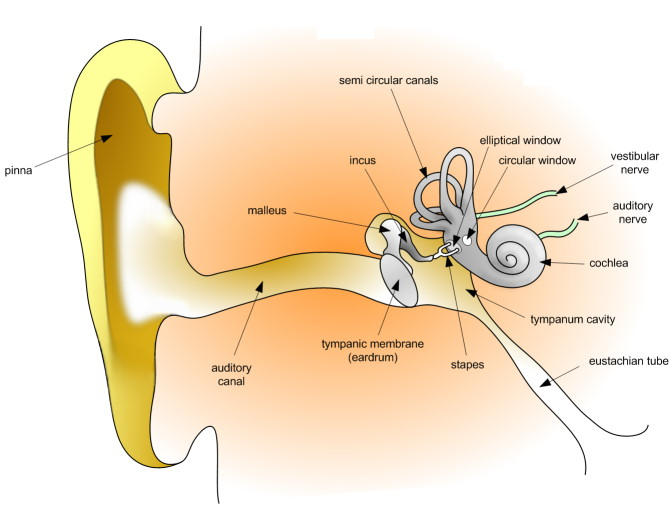
\includegraphics{HumanEar}
  \caption{Diagram of the auditory system of the human ear. Image source: SASOL Inzalo Foundation.}
\end{figure}

\section{Noise Pollution}
Unwanted or unpleasant sound is called noise. When there is too much noise in our surroundings, it leads to noise pollution.

Common sources of noise pollution include traffic noise from vehicles and horns, loudspeakers used at high volume,industrial noise from machines and factories, construction activities.

Continuous exposure to loud noise can cause stress, lack of sleep, and hearing problems. How can we reduce noise pollution?

We can reduce noise pollution by avoiding unnecessary honking on the roads, keeping the volume of loudspeakers low, using silencers and maintaining vehicles properly, planting trees, which can help absorb sound, following rules and regulations about noise levels.

Reducing noise pollution helps create a healthier and more peaceful environment.

\section{Hearing loss and hearing aids}
Sounds above 85 dB (such as loud headphones, factory machines, or heavy traffic) can bend and snap the delicate hair cells inside the cochlea. Broken hair cells cannot regrow. Hearing aids are devices that help by amplifying incoming sound waves so remaining hair cells can detect them.
\begin{marginfigure}
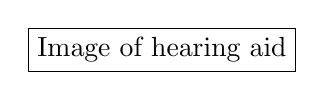
\begin{tikzpicture}
  \node[draw] at (0,0) {Image of hearing aid};
\end{tikzpicture}
  \caption{Image of hearing aid}
\end{marginfigure}

\section{}
When you listen to an audio recording of your voice, sound reaches your ears strictly through air conduction. The sound propagates from the speaker through air into our ear canal. When you speak live, sound reaches your inner ear through two paths at once. One, the sound propagates out of our mouth and around to our ears, and two, vibrations from the mouth also spread directly through our jaw and skull bones to our inner ear. Our skull bones lower the pitch of vibrations, making your voice sound deeper to you while speaking than it does on a recording!

\marginnote{If you pick up a seashell on a beach and hold it close to your ear, you may hear a sound that resembles waves breaking on the shore. Where does this sound come from?}

\subsection{Ultrasound}
Humans can hear sounds with frequencies roughly between 20 \hertz and 20,000 \hertz. Sounds with frequencies higher than 20,000 \hertz are called ultrasound. Humans cannot hear ultrasound.

Ultrasound has many useful applications:

\begin{enumerate}
\item Medical imaging: Doctors use ultrasound to look inside the body, for example to observe a developing fetus during pregnancy.
\item Detecting cracks in materials: Ultrasound can be used to find cracks or defects in metals and other materials.
\item Animal communication and navigation: Some animals, such as bats and dolphins, produce and detect ultrasound. They use it to communicate and to find objects around them.

\begin{marginfigure}
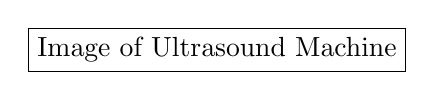
\begin{tikzpicture}
  \node[draw] at (0,0) {Image of Ultrasound Machine};
\end{tikzpicture}
\caption{Image of Ultrasound Machine}
\end{marginfigure}

\begin{marginfigure}
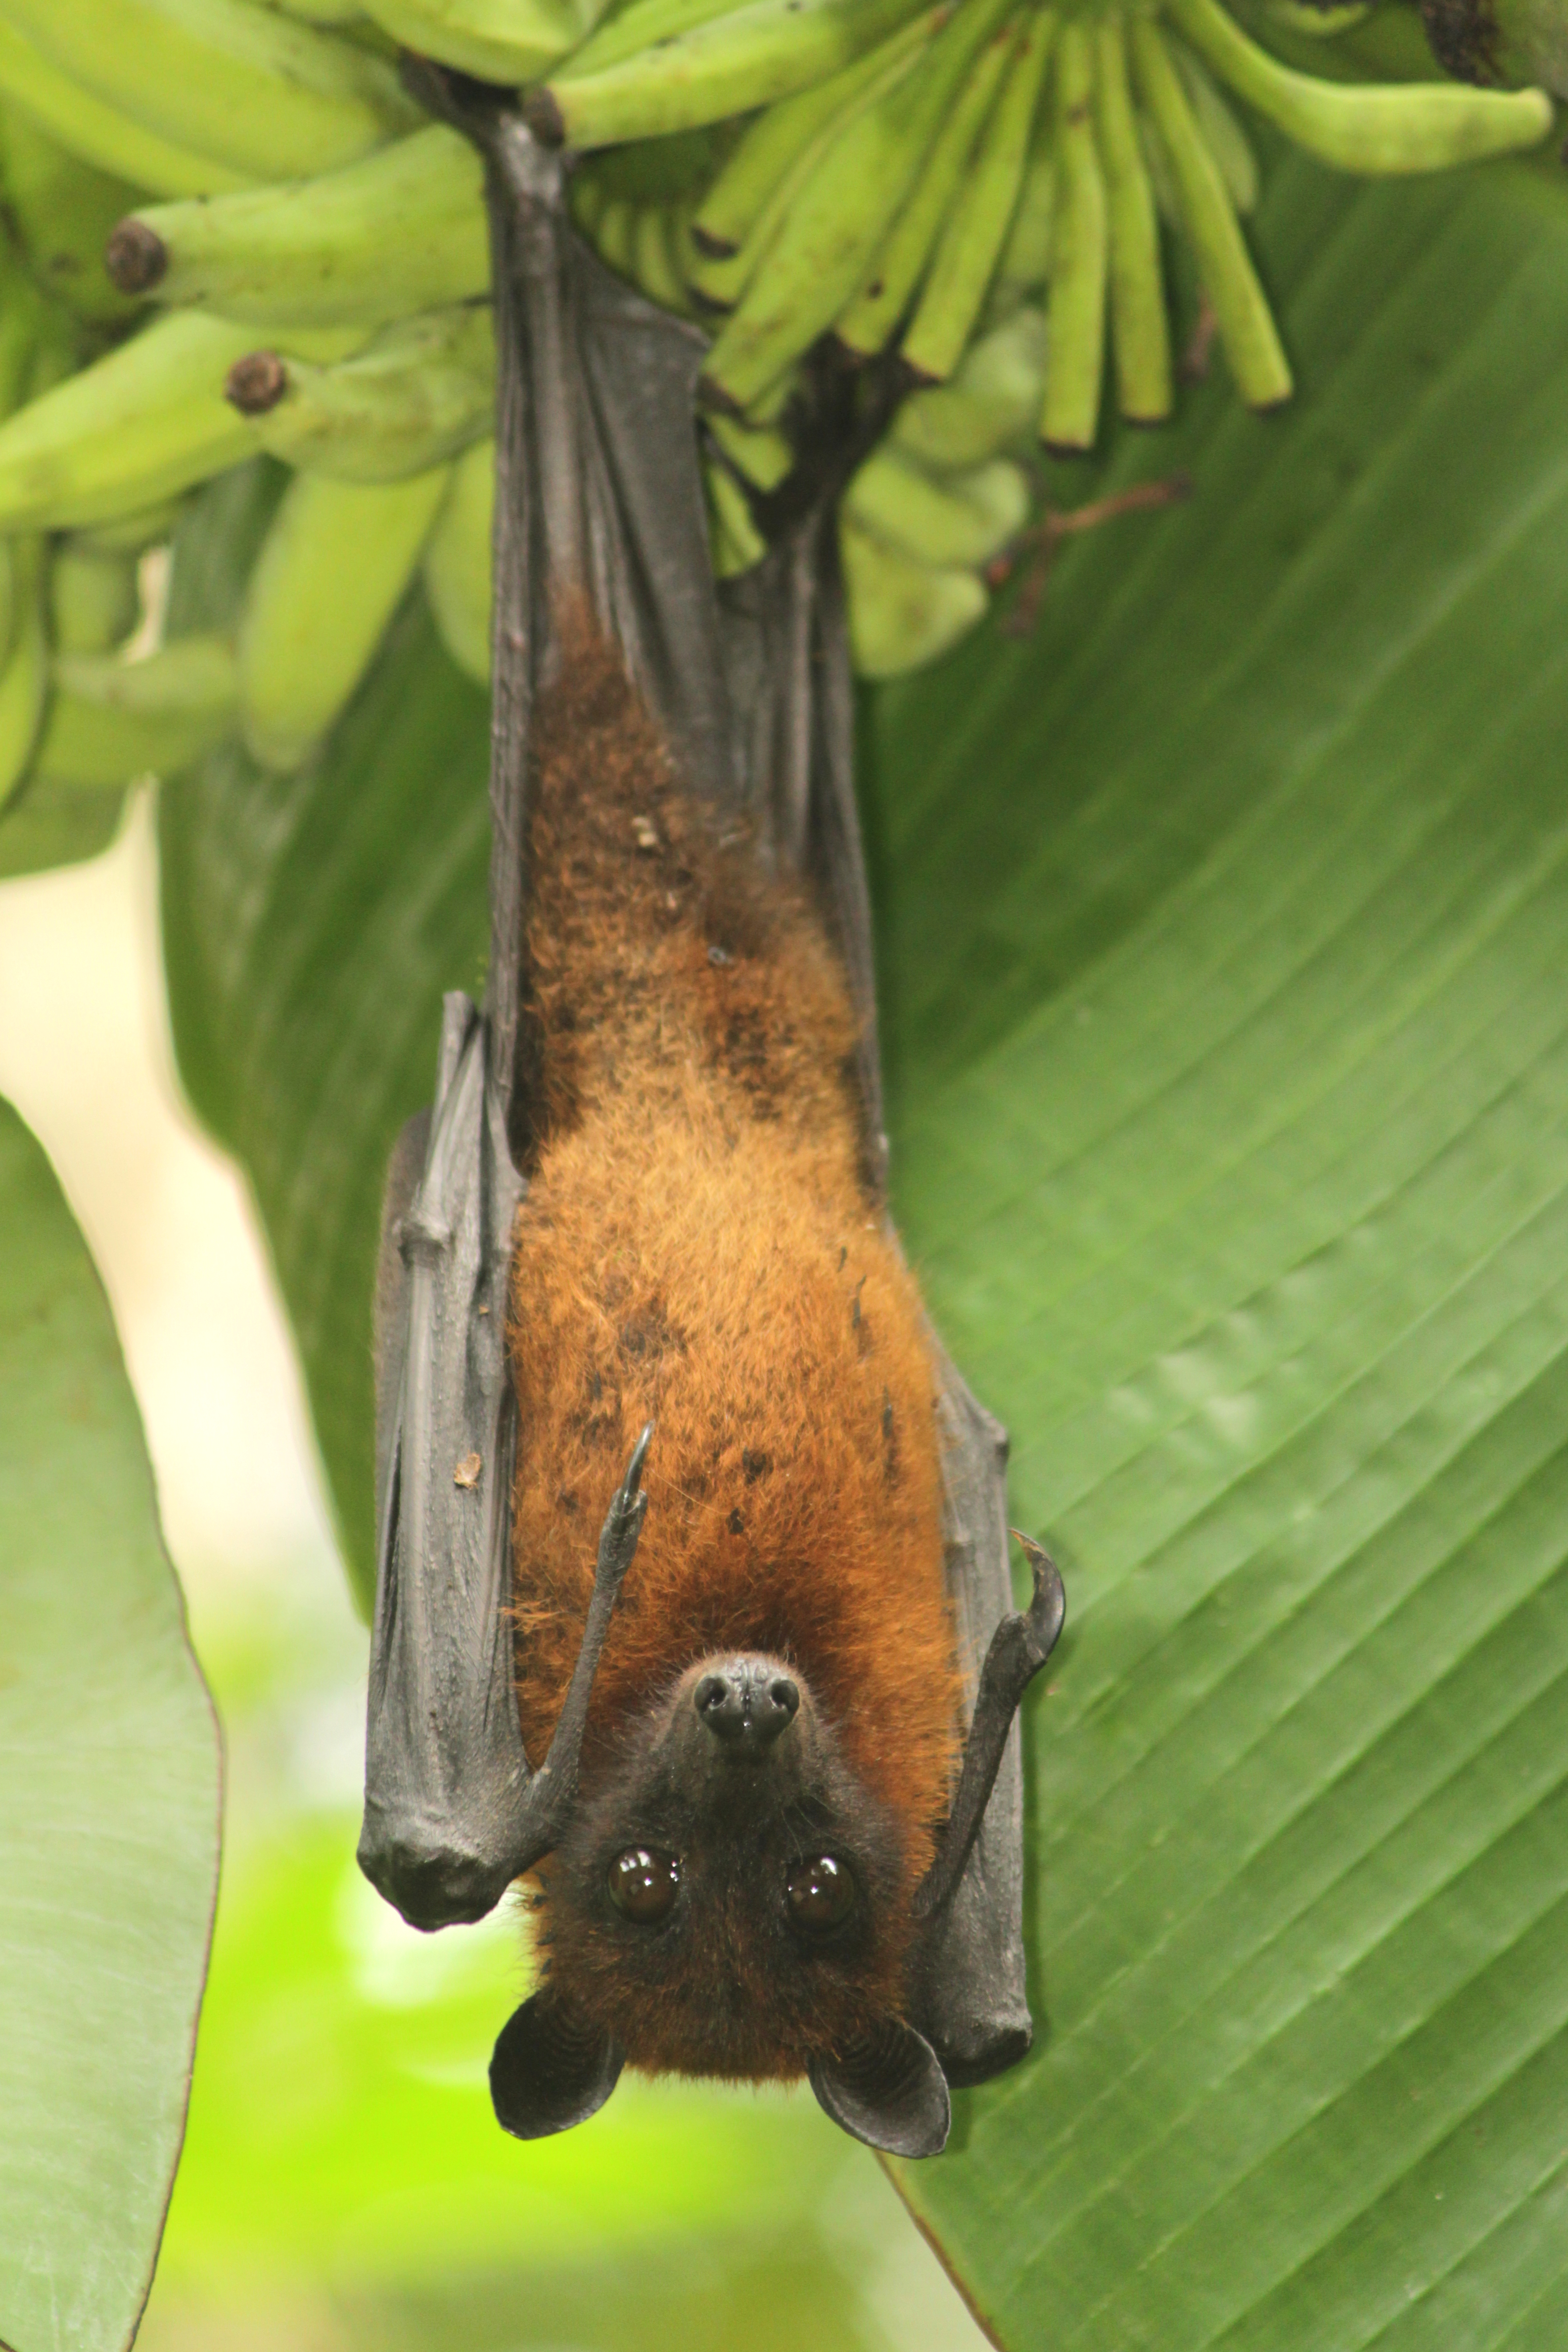
\includegraphics{bat}
\caption{Greater Indian fruit bat, image by Praveenp, licensed under CC BY-SA 4.0}
\end{marginfigure}
\end{enumerate}
\subsection{Echo}
Sound travels at a finite speed. When a sound wave meets a surface such as a wall, cliff, or building, it can reflect and travel back toward the source.

An echo is heard when the reflected sound reaches our ears after a short delay.

For an echo to be heard clearly, the reflecting surface must be far enough away. If the surface is too close, the reflected sound mixes with the original sound and we do not hear a separate echo.

For example, when you shout in a large empty hall, valley, or near a cliff, you may hear your own voice repeated after a short time. This repeated sound is the echo. Echoes show that sound waves can reflect from surfaces and travel back to us.
\begin{figure}[h!]
  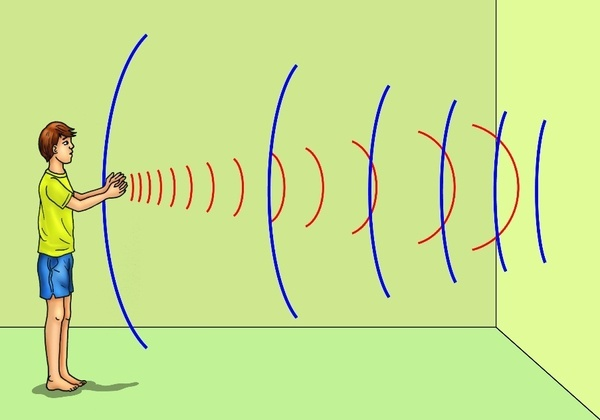
\includegraphics{echo}
  \caption{Image source: SASOL Inzalo Foundation}
\end{figure}
Big halls use sound-absorbing materials on walls and ceilings such as heavy carpets, padded seats, and perforated wood panels to stop unwanted echoes and make speech clear.

\subsection{Echolocation}
Animals such as bats and dolphins produce sounds and listen to the echoes to locate objects around them.
\subsection{Sonar}
Ships and submarines use sound waves and their echoes to detect objects underwater and measure distances.


\subsection{}
Sound is an example of a mechanical wave. It is also a longitudinal wave, because the particles of the medium vibrate along the direction in which the wave propagates. There is another type of wave called a transverse wave. In a transverse wave, the particles of the medium move perpendicular to the direction in which the wave propagates. In other words, the particles move up and down, while the wave moves forward.

An example of a transverse wave can be seen when a pebble is dropped into a pond. The ripples that spread across the surface of the water are transverse waves.

Light is also a transverse wave. However, light does not need a material medium to propagate, so it is not a mechanical wave.

The world around us is full of waves - sound waves, water waves, and light waves.
% ---------------------------------------------------------------------------------
% ---------------------------------------------------------------------------------
\end{document}
Consider the case of a vibrating string. When the string vibrates, it pushes and pulls the particles around it. These particles push and pull the particles next to them. In this way, the disturbance moves through the medium. See Figure~\ref{fig:vibrating-string}.
\begin{figure}
  \begin{tikzpicture}
    \node at (0,0) {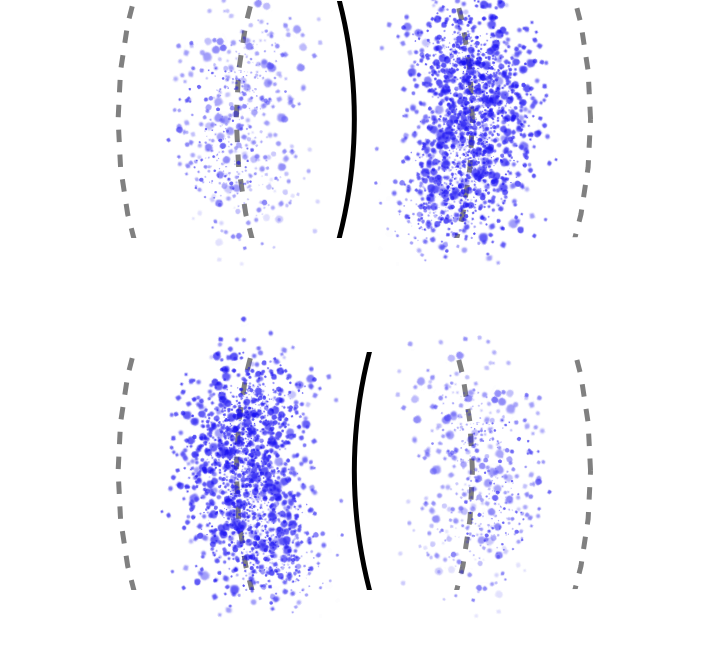
\includegraphics[width=10cm]{vibrating-string}};
    \draw (0,0) -- (0,0.5) node {String};
    \draw (0,1.5) -- (0,1);
    \draw (0,5) -- (3,5) node [midway] {Compression (high pressure)};
    \draw (-2,5) -- (0,5) node [midway] {Rarefaction (low pressure)};
    \draw (-2,-4) -- (0,-4) node [midway] {Rarefaction (low pressure)};
    \draw (0,0) grid (5,5);
  \end{tikzpicture}
  \caption{\label{fig:vibrating-string}Sound wave propagates from the source of sound (drum in this case) to the listener in the form of vibrations in the medium.}
  
\end{figure}





In such waves, the particles of the medium move parallel to the direction in which the wave propagates. Such waves are called \textbf{longitudinal waves}. Sound propagates as a longitudinal wave through solids, liquids, and gases.


\subsection{Compressions and Rarefactions}
When sound propagates through air, the air particles move back and forth around their positions. As they move, the particles sometimes come closer together and sometimes move farther apart. Regions where the air particles are closely packed are called \textbf{compressions}. Regions where the particles are farther apart are called \textbf{rarefactions}. See Figure~\ref{fig:compressionRarefaction}.

As a sound wave propagates, compressions and rarefactions move forward through the air. This pattern of compressions and rarefactions carries sound from the source to our ears.


\section{Frequency of Sound}
\subsection{Activity: Vibrating Scale}
Place a scale on the edge of a desk so that part of it stays over the edge. Hold the scale firmly on the desk and pluck the free end so that it vibrates and produces a sound. Optionally, you may record a slow-motion video using a phone.









\newthought{Question:} A bell is struck and produces sound. After a few seconds, the sound stops. What must have happened to the bell?

\newthought{Question:} Kavin and Priya are standing at different distances from the lightning. Both hear the thunder. Will the pitch of the thunder be different for them? Will the loudness of the thunder be different?


\subsection{Activity: Long spring}

Take a long spring. Ask your classmate to hold one end while you hold the other end. Stretch the long spring gently between you. Now give the long spring a quick push toward your classmate.

\newthought{Observe:} You will see regions where the coils are close together and regions where they are farther apart. A region where the coils are close together is called a compression. A region where the coils are farther apart is called a rarefaction. This is similar to what happens in sound waves in air.





\subsection{Musical instruments}
Musical instruments produce sound by making strings, membranes, or air columns vibrate. By changing certain parts of the instrument, musicians can change the frequency of vibration, and therefore the pitch of the sound.

Different instruments change the frequency in different ways.

Veena (string instrument): The strings vibrate to produce sound. Pressing the string at different positions changes the length of the vibrating string, which changes the frequency and the pitch.
\begin{marginfigure}
  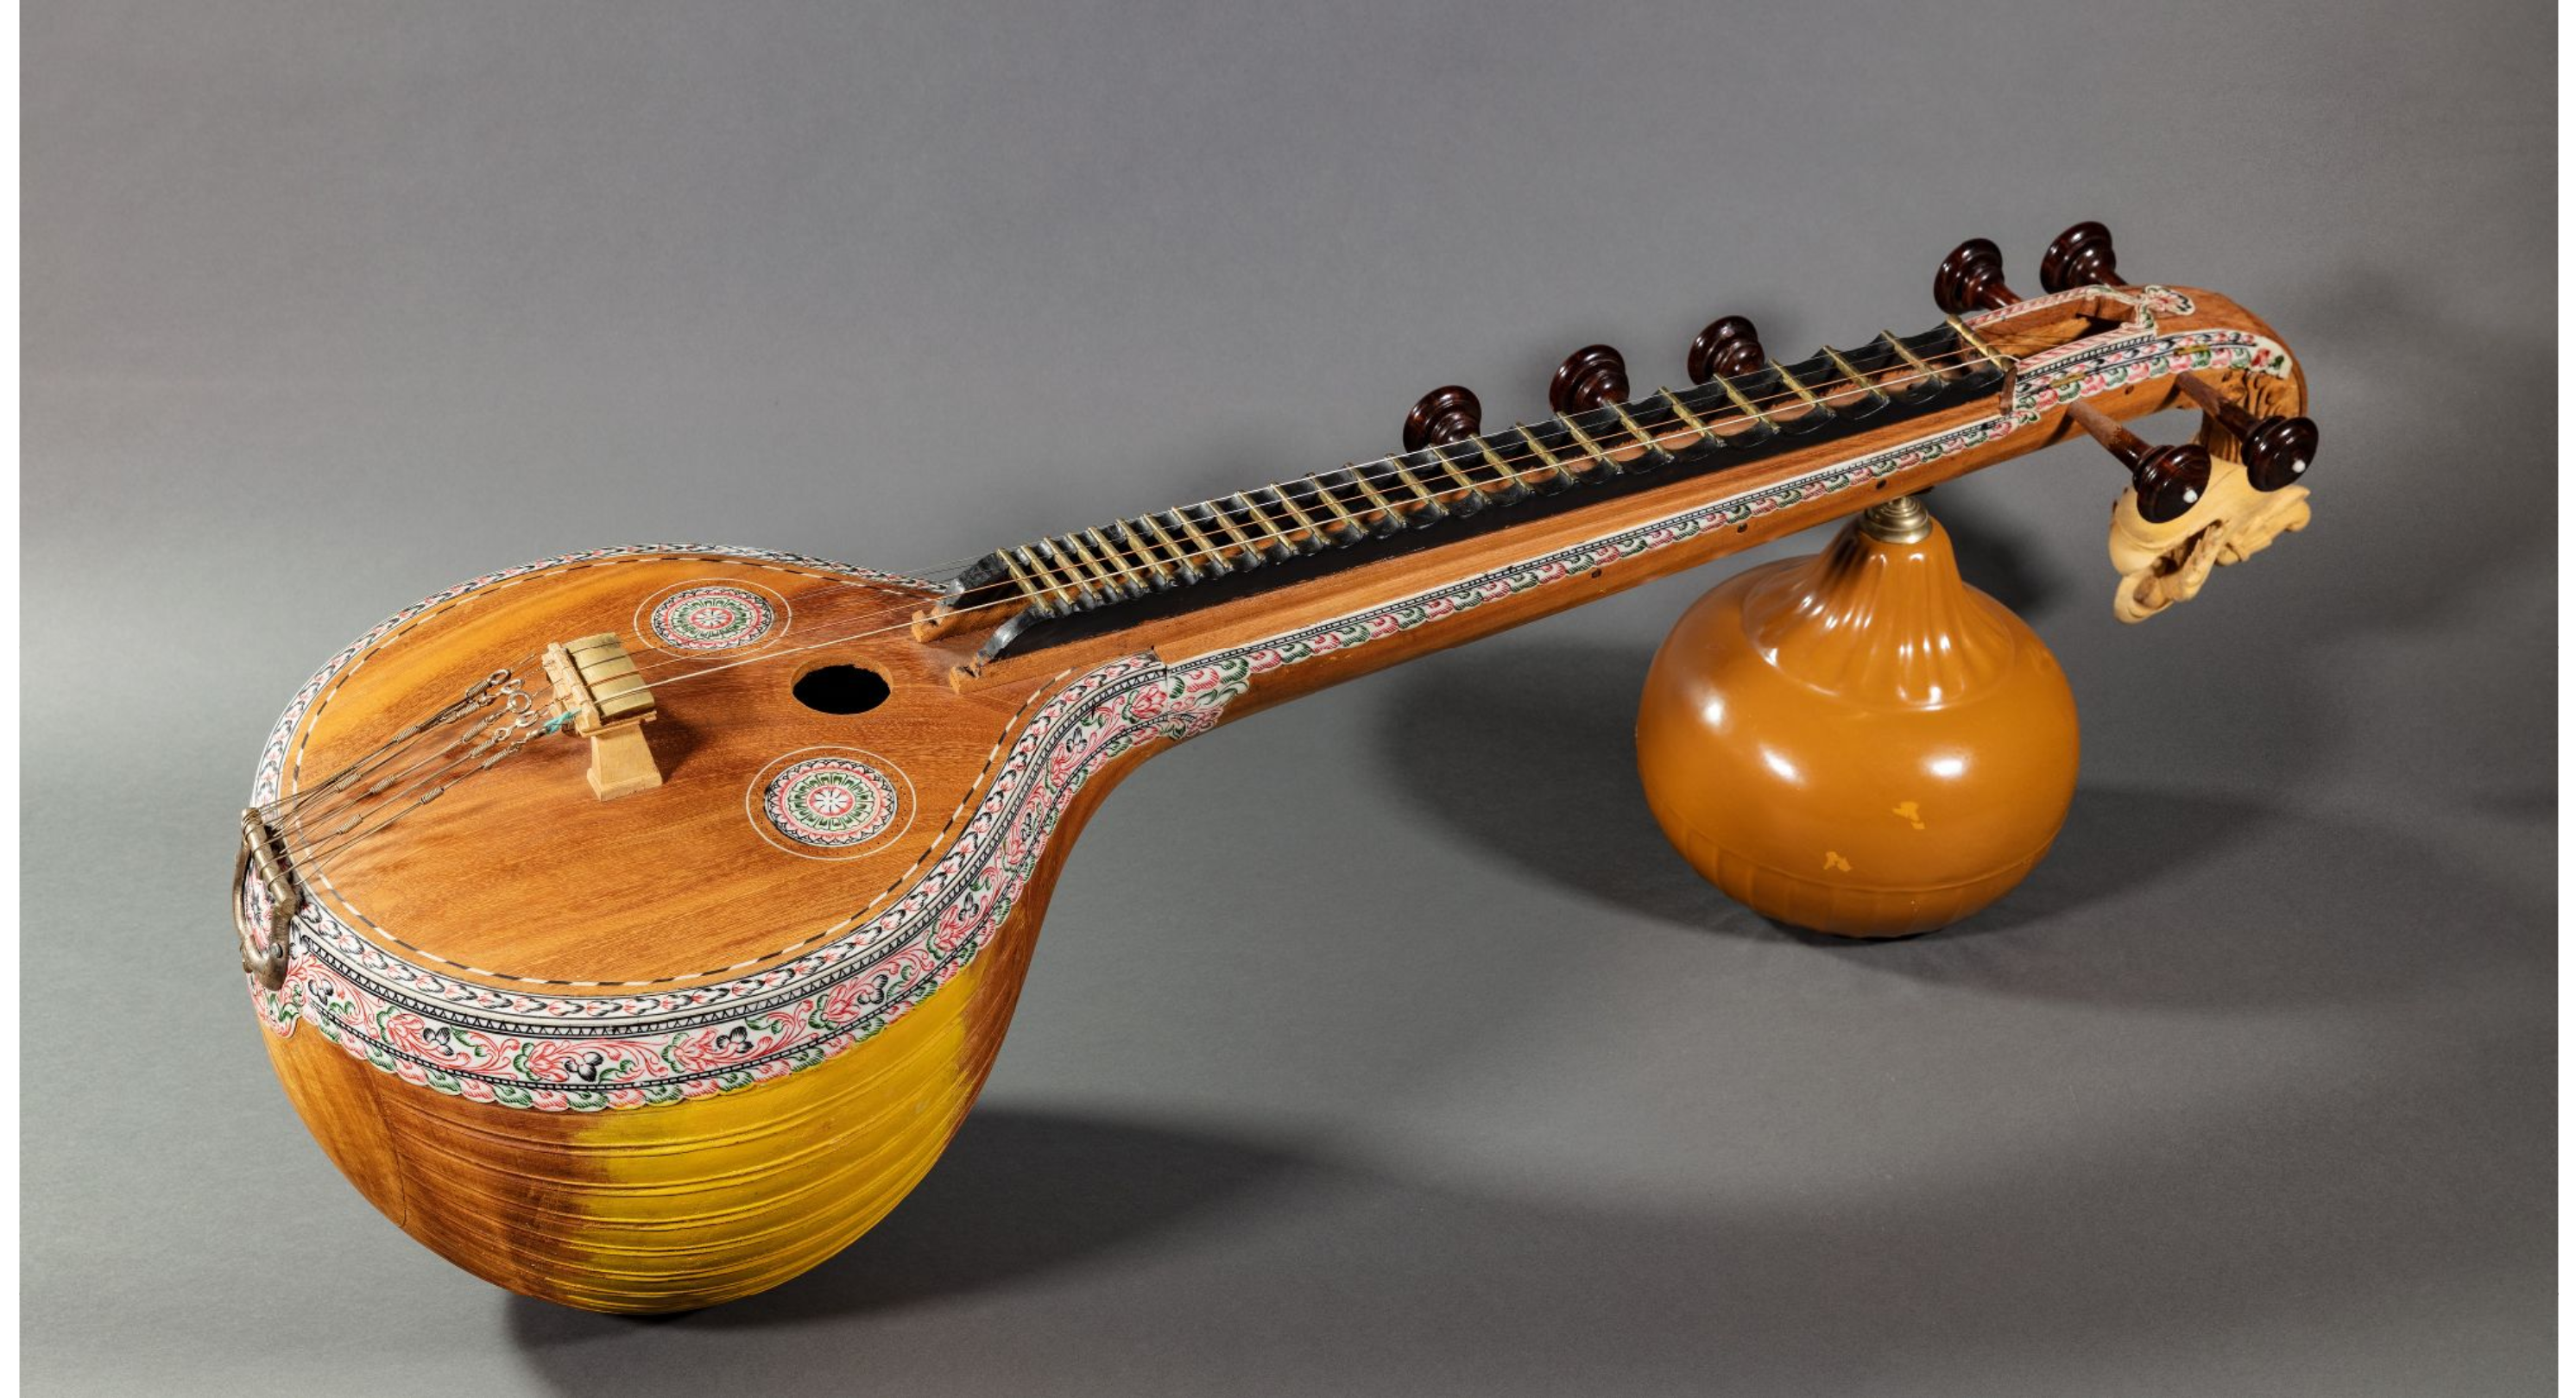
\includegraphics{veena}
  \caption{Veena from Chennai, Wikimedia Commons}
\end{marginfigure}

Parai (drum): The stretched membrane (skin) vibrates when it is struck. Changing the tightness of the membrane changes the frequency of vibration and the sound produced.
\begin{marginfigure}
  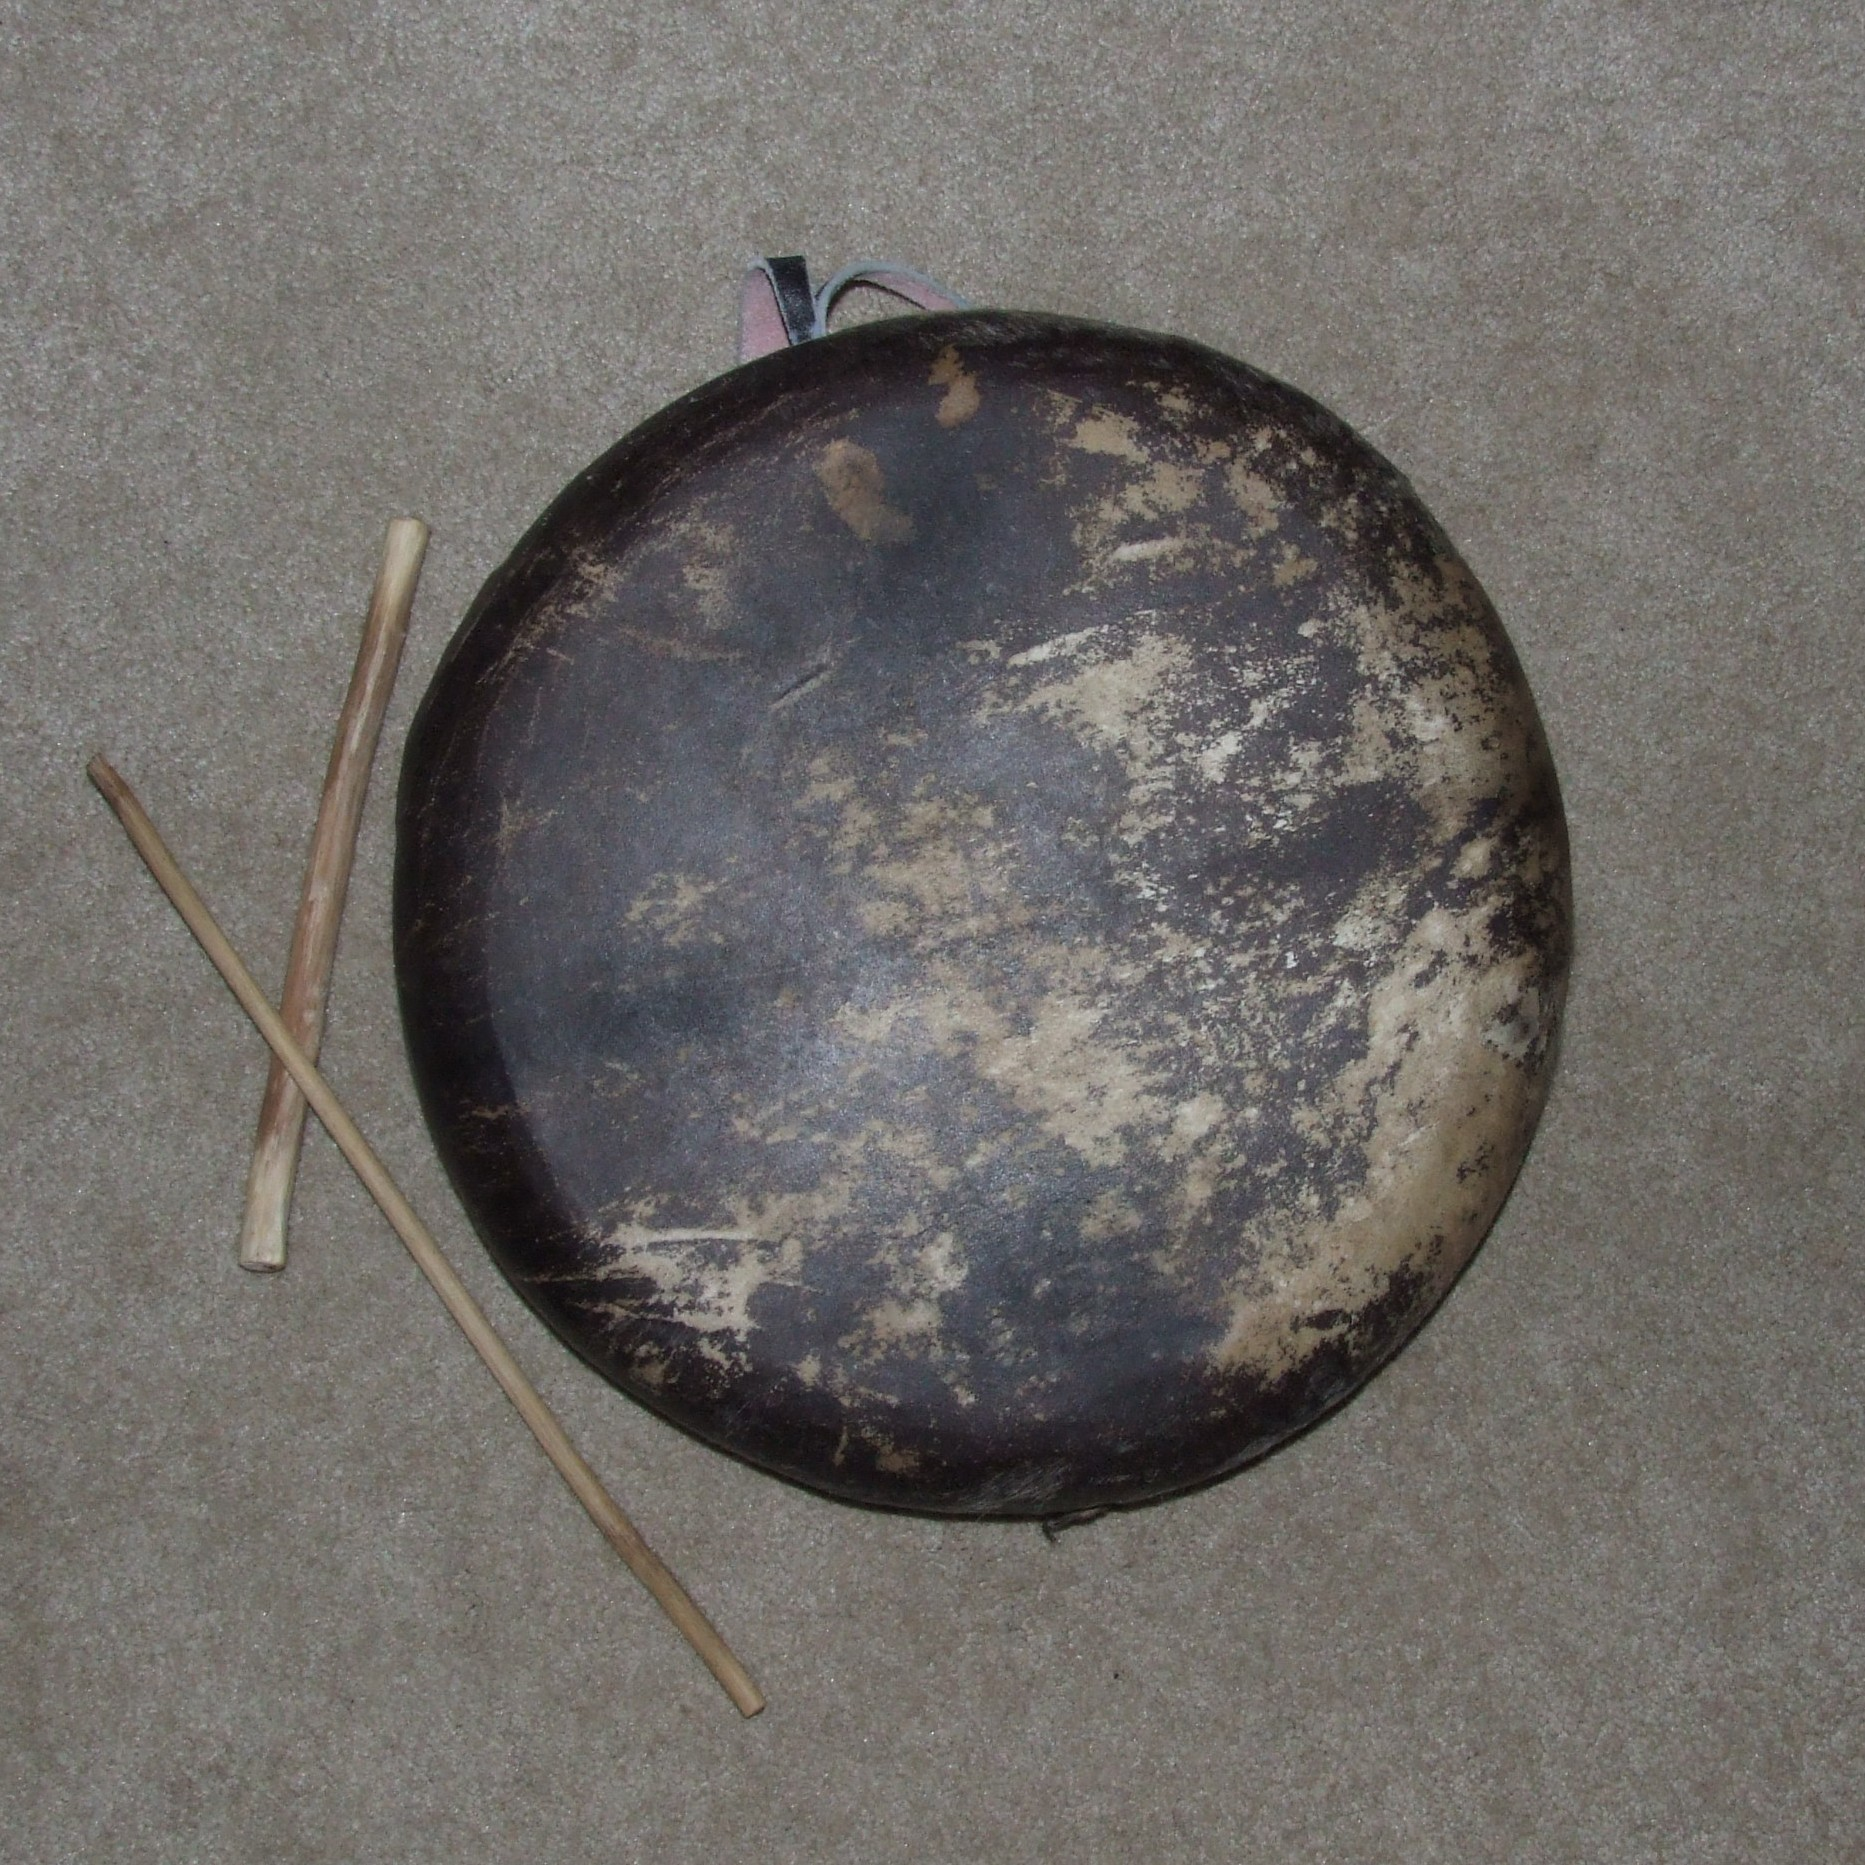
\includegraphics{parai}
\caption{Front side of a parai with the sticks used to play the instrument. Image by Prabhunkl, licensed under CC BY-SA 4.0}  
\end{marginfigure}
Nadaswaram (wind instrument): Sound is produced by vibrations of the air column inside the instrument. Opening and closing the finger holes changes the effective length of the air column, which changes the frequency.
\begin{marginfigure}[-25\baselineskip]
  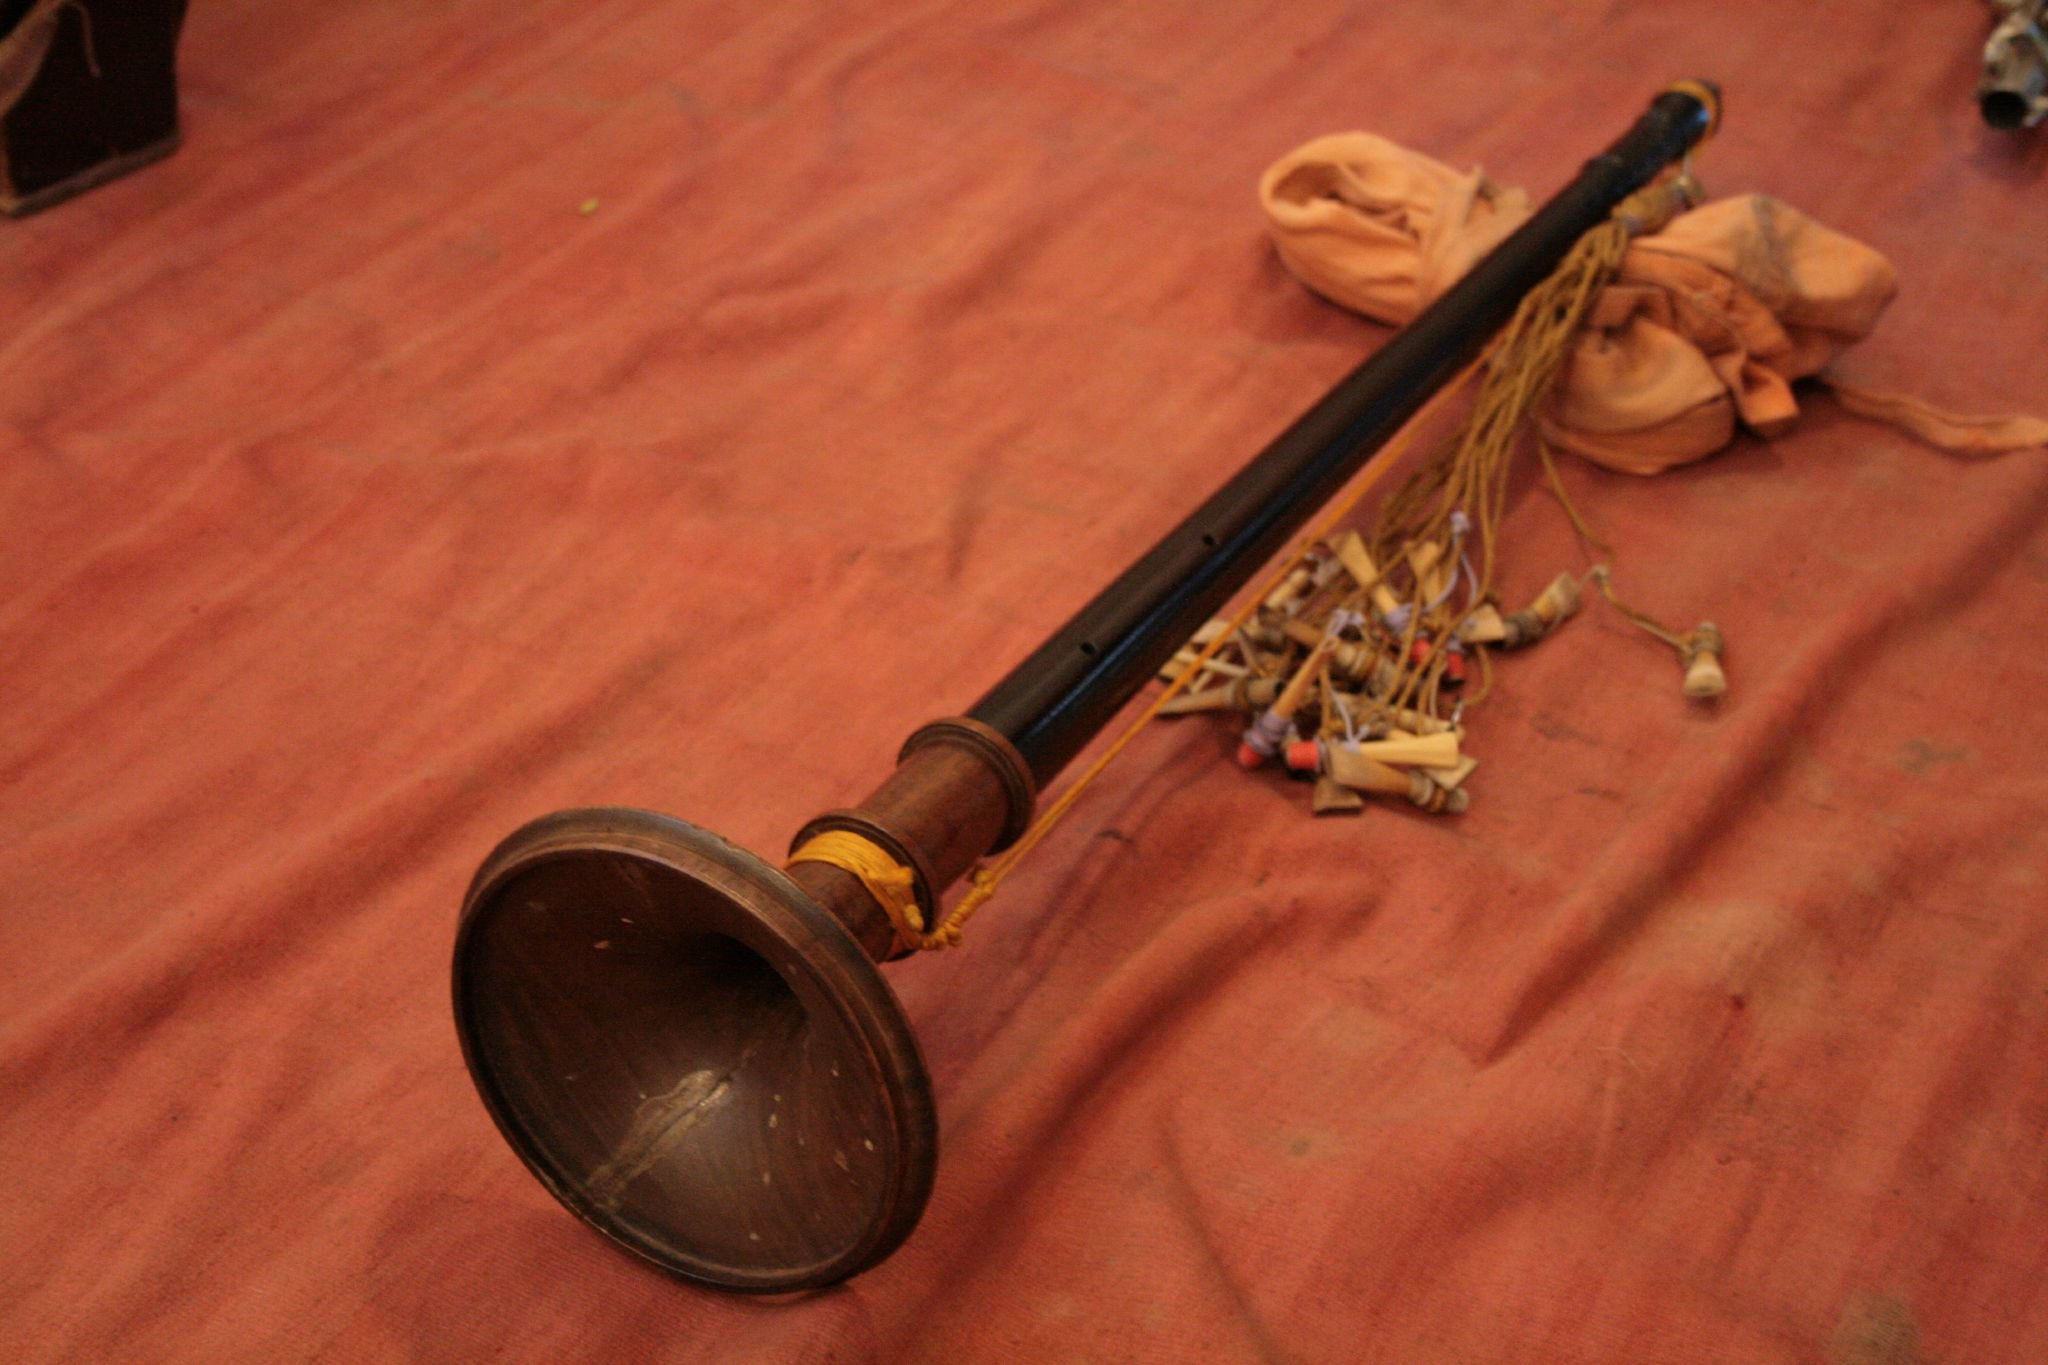
\includegraphics{nadaswaram}
\caption{Nadaswaram (also nagaswaram or nagasuram), Image by Ashwin Kamath}
\end{marginfigure}
Although these instruments look very different, they all produce sound through vibrations, and the frequency of vibration determines the pitch of the sound.




% \newpage
% \nocite{halliday2013fundamentals}
% \nocite{walker2006flying}
% \nocite{PhysRevSTPER.6.020114}

% \bibliographystyle{plainnat}
% \bibliography{sound}


Similarly, the particles in the medium do not travel all the way from the sound source to our ears. They move back and forth around their usual positions. A disturbance that travels through a medium in this way is called a \textbf{wave}. Sound propagates through air as a sound wave. 